\documentclass[11pt]{article}
\usepackage[T1]{fontenc}
\usepackage[utf8]{inputenc}
\usepackage{mathpazo}
\usepackage{amsmath,amssymb,amsthm,mathtools}
\usepackage[margin=1.05in]{geometry}
\usepackage{microtype}
\usepackage{enumitem}
\usepackage{booktabs,array}
\usepackage{graphicx,xcolor}
\usepackage{placeins}
\usepackage{tikz}
\usetikzlibrary{calc,arrows.meta,positioning,decorations.pathreplacing}
\usepackage{xurl}
\usepackage[colorlinks=true,linkcolor=blue!45!black,citecolor=blue!45!black,urlcolor=blue!45!black]{hyperref}
\usepackage[capitalise,noabbrev]{cleveref}
\hypersetup{pdftitle={A hyperbolic group with no geometric CAT(0) action},pdfauthor={OpenAI},bookmarksdepth=2}
\newtheorem{theorem}{Theorem}[section]
\newtheorem{proposition}[theorem]{Proposition}
\newtheorem{lemma}[theorem]{Lemma}
\newtheorem{corollary}[theorem]{Corollary}
\theoremstyle{definition}
\newtheorem{definition}[theorem]{Definition}
\theoremstyle{remark}
\newtheorem{remark}[theorem]{Remark}
\newcommand{\CAT}{\operatorname{CAT}}
\newcommand{\E}{\mathbb E}
\newcommand{\Prob}{\mathbb P}
\newcommand{\F}{\mathbb F}
\newcommand{\R}{\mathbb R}
\newcommand{\Z}{\mathbb Z}
\newcommand{\ip}[2]{\langle #1,#2\rangle}
\newcommand{\norm}[1]{\lVert #1\rVert}
\DeclareMathOperator{\barc}{bar}
\DeclareMathOperator{\supp}{supp}
\DeclareMathOperator{\diam}{diam}
\DeclareMathOperator{\TV}{TV}
\setlist{topsep=4pt,itemsep=3pt,parsep=0pt}
\setlength{\emergencystretch}{1.5em}
\numberwithin{equation}{section}
\pdfminorversion=5
\ifdefined\pdfinfoomitdate\pdfinfoomitdate=1\fi
\ifdefined\pdftrailerid\pdftrailerid{}\fi

\title{A hyperbolic group with no geometric CAT(0) action}
\author{OpenAI}
\date{September 25, 2026}
\begin{document}
\maketitle
\begin{abstract}
We construct a hyperbolic group with a finite classifying space that admits no geometric action on a proper complete CAT(0) space. Consequently, a finite aspherical simplicial complex with a linear combinatorial disk-filling inequality need not have a finite locally CAT(0) homotopy model, and hence need not have a finite locally CAT($-1$) model. Here metric models carry geodesic length metrics inducing the given complex topology.
\end{abstract}
\setcounter{tocdepth}{1}
\tableofcontents
\clearpage
\section{Introduction}\label{sec:introduction}
A linear isoperimetric inequality is a large-scale expression of negative curvature: for finitely presented groups, it characterizes word hyperbolicity. Local comparison geometry is more restrictive. The geometric realization question asks whether every hyperbolic group admits a geometric action on a proper $\CAT(0)$ space, or on a proper $\CAT(-1)$ space. We construct a group for which neither action exists.

Throughout the paper, a \emph{geometric action} is a proper, cocompact action by isometries, and metric models of finite complexes carry geodesic length metrics inducing the given complex topology.

\begin{theorem}\label{thm:main}
There exist a finite connected two-dimensional aspherical simplicial complex $K$ and a constant $C<\infty$ with the following properties.
\begin{enumerate}[label=\textup{(\roman*)}]
\item Every combinatorial edge loop of length $\ell$ in the universal cover of $K$ bounds a disk diagram with at most $C\ell$ triangular faces.
\item The group $\pi_1K$ admits no geometric action on a proper complete $\CAT(0)$ space.
\end{enumerate}
In particular, $\pi_1K$ is word-hyperbolic, and no finite simplicial complex homotopy equivalent to $K$ admits a locally $\CAT(0)$ geodesic length metric inducing its given topology. Consequently, no such model admits a compatible locally $\CAT(-1)$ geodesic length metric.
\end{theorem}

The proof is an existence argument and does not give an effective size for $K$. The filling constant may depend on the selected finite presentation.

\subsection{Context}
The realization problem goes back to the development of hyperbolic groups.
In his account of that development, Gromov recalls introducing linear
isoperimetry as a group-theoretic form of negative curvature and then
spending years seeking geometric realizations by negatively curved
spaces~\cite[p.~396]{RaussenSkau2010}.
The equivalence between linear filling and word hyperbolicity became
part of the foundational theory~\cite{Gromov1987}; see also
\cite[Theorem~III.$\Gamma$.2.6 and Remark~III.$\Gamma$.2.7(2)]{BH1999}.
The $\CAT(-1)$ realization question appears as Problem~H11 in
Baumslag--Myasnikov--Shpilrain's 1999 problem
list~\cite{BaumslagMyasnikovShpilrain1999}.
Both the $\CAT(-1)$ and $\CAT(0)$ questions appear as open problems
in Stark's 2025 survey~\cite[Open Problem~2.15]{Stark2025} and in the
March 2026 preprint of Duchesne--Simon~\cite[Question~W]{DuchesneSimon2026}.

There are several successful ways to obtain such geometric actions.
Finitely generated free groups act on trees and closed hyperbolic manifold groups act on
hyperbolic space. More generally, a finite complex carrying a locally
$\CAT(-1)$ or locally $\CAT(0)$ geodesic length metric inducing its topology has a universal cover
with the corresponding global curvature bound; its deck action is
geometric~\cite[Theorem~II.4.1]{BH1999}.
Cubulation provides another route to $\CAT(0)$ models.
For example, Ollivier--Wise prove that random groups in the density
model at density less than $1/6$ act freely and cocompactly on
$\CAT(0)$ cube complexes with probability tending to one as relator
length grows, with the number of generators fixed~\cite[Theorem~10.4]{OllivierWise2011}.
Thus random presentations can produce geometric $\CAT(0)$ actions as
well as hyperbolicity; the relations used here must enforce an
additional obstruction.

Dimension restrictions already yield obstructions.
Brady--Crisp~\cite[Theorem~2]{BradyCrisp2007} construct infinitely many
torsion-free hyperbolic groups of geometric dimension two which admit
no proper isometric action on a proper two-dimensional $\CAT(0)$
space. Their Theorem~1 gives a hyperbolic group of $\CAT(0)$ dimension
two and $\CAT(-1)$ dimension three. These conclusions rely on
constraints on translation lengths in two-dimensional targets.
Theorem~\ref{thm:main} excludes geometric $\CAT(0)$ actions in every
dimension. Its finite-model consequence also allows the entire
simplicial complex to change within its homotopy type: any compatible
locally $\CAT(0)$ geodesic length metric on such a model would recover a geometric
action by passing to the universal cover.

Random-presentation proofs of hyperbolicity combine counting for
bounded diagrams with a local-to-global argument.
Our treatment of repeated relator occurrences is related to the
multiplicity and constraint methods in
Ollivier~\cite[Section~2.2]{Ollivier2004} and
Antoniuk--Friedgut--\L uczak~\cite[Section~3]{AntoniukFriedgutLuczak2017}.
Within each finite presentation we first sample small labelled graphs,
then larger labelled graphs whose required small graphs have already
been selected. The same prerequisite can support several larger
graphs, so its probability cost must be charged only once.
Section~\ref{sec:diagrams} proves the resulting estimate directly.

The obstruction to actions uses the harmonic-energy framework of
Gromov~\cite[Sections~3.3 and~3.7]{Gromov2003} and
Izeki--Nayatani~\cite{IzekiNayatani2005}.
In this framework, expansion in a finite graph can force a fixed point
when the target satisfies a suitable nonlinear spectral inequality.
The target hypothesis matters: Izeki--Kondo--Nayatani obtain random
hyperbolic groups with fixed-point properties for target classes whose
tangent-cone invariant is bounded by a prescribed constant strictly
less than one~\cite[Corollary~3.8]{IzekiKondoNayatani2012}.
Toyoda~\cite[Theorem~1.4]{Toyoda2016} supplies such spectral bounds
for a prescribed finite family of geodesically complete $\CAT(0)$
spaces admitting proper cocompact actions, with constants depending
on that family.
Here a hypothetical target and its action can be chosen after the
finite presentation is known. We obtain the required uniformity from
bounds on every generator displacement and total-variation couplings
of table matches. Sturm's inductive
means~\cite[Definition~4.6 and Theorem~4.7, proof~(a)]{Sturm2003}
then turn those couplings into the averaging estimate used in the
energy argument.

\subsection{Structure of the proof}
The construction must satisfy two requirements: its relations must be sparse
enough to preserve hyperbolicity and asphericity, yet impose enough metric
constraints to exclude geometric actions on proper $\CAT(0)$ spaces.
We organize the relations using a fixed modification of the incidence graph
of the projective plane over $\mathbb F_2$.  Four point vertices are doubled.
At one of them we omit one incidence and keep its counterpart at the other
representative separate.  The remaining edges over each point form a small
connected graph, called a fan.  We call the resulting incidence graph
the core.  Edges receive signed generator labels,
and every closed walk in a selected labelled graph gives a relation.
Fans are selected first; a labelled copy of the whole graph is selected only
when its seven fan restrictions have already been selected.  We study
copies for which further four-letter relations close every nonbacktracking two-edge core
path to a square.  An independent collection of six-letter relations will
control individual generator displacements.  A labelled core copy together
with one chosen square completion for every nonbacktracking two-edge core path is a
\emph{match}.

We choose a sequence of such finite presentations, with progressively stronger
finite counting requirements.  At each stage, a finite list of statistical
tests is fixed before choosing the sampling parameters; those parameters then
remain fixed while the alphabet grows.  If infinitely many of their groups admitted
geometric actions on proper complete $\CAT(0)$ spaces, choose one
action for each of those groups.
The closed-walk relations realize the fixed graph by orbit points in every
chosen action.  After normalizing the average squared generator displacement,
products of these configurations have a limiting configuration in a complete
$\CAT(0)$ space.  The counting requirements force exact metric identities in
that limit, and a finite geometric contradiction excludes it.  Thus every
sufficiently late group in the chosen sequence admits no such action.  The argument uses the following three ingredients.

\begin{enumerate}
\item \textbf{A positive deficit in diagram counting.}
A fan shared by several copies of the whole graph supplies only one random
table entry, so its probability cost must be counted once.  At the same time,
a disk or sphere diagram may use the same relation many times.  We reconcile
these two counts by assigning multiplicity weights to distinct table entries.
Local incidence estimates at vertices then leave a positive multiple
of the diagram's area to be paid by its boundary.  This is first proved for
bounded fragments.  Planar separators extend it to all diagrams, yielding
both a linear filling inequality and asphericity in
Section~\ref{sec:diagrams}.

\item \textbf{Sampling that is uniform over later actions.}
The metric argument compares a bounded function of one or two edge labels
with a further edge label.  The relevant tuples need not have dense
projections in the sampled tables.  Instead, we couple several matches
so that the conditioning labels agree, each match is approximately
uniform among all matches, and the further labels are approximately independent
uniform generators.  Section~\ref{sec:sampling} obtains this coupling by
gluing copies along an enlarged conditioning tuple and proving concentration
of the numbers of extensions.  The enlargement is chosen by counting
exponents so that every further collection of label positions has a strictly positive
margin.  The conclusions concern total variation of finite probability laws.  They therefore apply to bounded tests from any action
chosen after the tables are revealed.  The common conditioning tuple may still depend on the further labels; the
averaging estimate allows this dependence.  The six-letter relations supply
the uniform displacement bound that makes these tests bounded.

\item \textbf{A rigid configuration and incompatible scalar products.}
Energy minimization and the coupling yield lower bounds for squared orbit
distances along short paths.  In the limit, the decoration squares force
squared two-step distances to equal two.  The six-cycles through three noncollinear point vertices then have a
common center, and their central triangles are flat
(Section~\ref{sec:energy}).  The doubled points give four unit vectors obtained
by doubling certain midpoints in the tangent cone at that center.  The line
incidences force two of these vectors to have nonnegative scalar product.
A three-field test involving the separated incidence edge forces the other
two vectors to be antipodal.  Splitting the parallel set of the resulting line exposes a flat
square in the transverse factor, which makes the first pair antipodal as well.
Their scalar product is consequently $-1$, the contradiction in
Section~\ref{sec:obstruction}.
\end{enumerate}

Section~\ref{sec:model} defines the finite graph and its random tables.
Section~\ref{sec:completion} makes the finite-test selection precise and
transfers one resulting finite classifying complex to the simplicial model
in Theorem~\ref{thm:main}.  Its filling constant may depend on that chosen
presentation.

\subsection{Conventions}
A disk diagram may have boundary spurs or edges collapsed to the target's $1$-skeleton; such features have zero area and can be removed. Its area is the number of its noncollapsed $2$-cells. Constants in filling estimates may depend on a fixed finite presentation. A statement holds \emph{with high probability} if its probability tends to one as the alphabet size tends to infinity, with all parameters in that statement fixed. Finite-test limits and the final diagonal selection will always be distinguished.

We use completed tangent cones and completed spaces of directions. The latter are $\CAT(1)$ and the former are $\CAT(0)$~\cite[Theorem~II.3.19]{BH1999}. For the tangent-cone construction in this generality, see also
Kleiner--Leeb~\cite[Section~2.1.3]{KleinerLeeb1997}, who credit
Nikolaev's tangent-cone theorem.
Subsequent products and limits need not be proper; properness is used only for the original geometric actions. Standard comparison, covering-space and topological results are cited with the hypotheses needed here. All estimates specific to the new construction are proved below.

\section{The incidence template and the nested tables}\label{sec:model}
We begin with the fixed finite combinatorics. All randomness will be in the labels, not in the template.

\subsection{Points, lines, and fans}
\begin{definition}[The incidence template]\label{def:template}
Identify the points of the projective plane over $\F_2$ with the seven nonzero vectors of $\F_2^3$. A line consists of the three nonzero vectors in a two-dimensional subspace. Fix
\[
 A=e_1,\qquad B=e_2,\qquad C=e_3,\qquad D=e_1+e_2+e_3.
\]
No three of these four points are collinear. For distinct points $i,j$, write $ij$ for their line.

The bipartite graph $\Gamma$ has a vertex $X_i$ for every point, an additional vertex $Y_i$ for $i\in\{A,B,C,D\}$, and a vertex for every line. Both representatives over a point are joined to each incident line, with one exception: the edge $Y_D$--$CD$ is omitted. The edge
\[
 e_0=X_D\text{--}CD
\]
is called the \emph{loose edge}. Every other edge belongs to the \emph{fan} $F_i$ at its point $i$. At $D$, the fan uses only the two lines other than $CD$, so $CD$ is not a vertex of $F_D$.
\end{definition}

Each $F_i$ is connected. At $A,B,C$ it is $K_{2,3}$, at $D$ it is $K_{2,2}$, and at each of the other three points it is a three-edge star. Let $g=7$ and $k_i=|E(F_i)|$. Thus
\begin{equation}\label{eq:model-counts}
 (k_i)_i=(6,6,6,4,3,3,3),\qquad
 \sum_i k_i=31,\qquad |E(\Gamma)|=32.
\end{equation}
The graph has $18$ vertices. Its cycle rank is $15$; the sum of the
cycle ranks of the fans is $7$. We will first impose the cycles within
the fans, then use a smaller graph of cycle rank $8$ to impose the
remaining core relations. The cone construction below makes this
decomposition explicit.

Figures~\ref{fig:fano-template} and~\ref{fig:fans} show the incidence
pattern and the exceptional fan.

\begin{figure}[htbp]
\centering
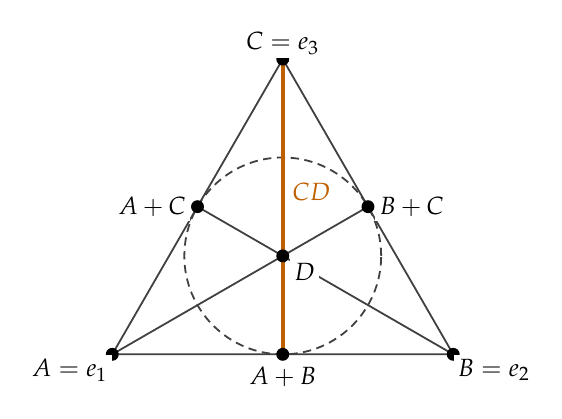
\begin{tikzpicture}[x=1.25cm,y=1.25cm,
  fano edge/.style={draw=black!75,line width=.65pt},
  fano point/.style={circle,fill=black,inner sep=1.65pt},
  fano label/.style={font=\small,fill=white,inner sep=1.5pt}]
  \coordinate (A) at ({-sqrt(3)},-1);
  \coordinate (B) at ({sqrt(3)},-1);
  \coordinate (C) at (0,2);
  \coordinate (D) at (0,0);
  \coordinate (AB) at (0,-1);
  \coordinate (AC) at ({-sqrt(3)/2},.5);
  \coordinate (BC) at ({sqrt(3)/2},.5);
  \draw[fano edge] (A)--(B)--(C)--cycle;
  \draw[fano edge] (A)--(BC) (B)--(AC);
  \draw[fano edge,densely dashed] (D) circle[radius=1];
  \draw[draw=orange!75!black,line width=1.35pt] (C)--(AB);
  \foreach \P in {A,B,C,D,AB,AC,BC}
    \node[fano point] at (\P) {};
  \node[fano label,anchor=north east] at (A) {$A=e_1$};
  \node[fano label,anchor=north west] at (B) {$B=e_2$};
  \node[fano label,anchor=south] at (C) {$C=e_3$};
  \node[fano label,anchor=north west] at (.07,-.03) {$D$};
  \node[fano label,anchor=north] at (0,-1.08) {$A+B$};
  \node[fano label,anchor=east] at ({-sqrt(3)/2-.07},.5) {$A+C$};
  \node[fano label,anchor=west] at ({sqrt(3)/2+.07},.5) {$B+C$};
  \node[fano label,anchor=west,text=orange!75!black] at (.05,.65) {$CD$};
\end{tikzpicture}
\caption{The seven points and seven lines of the Fano plane.  The three sides,
three medians, and dashed circle each represent one projective line; only
marked dots represent projective points.  The
points $A,B,C,D=A+B+C$ form a quadrangle: no three are collinear.  The thick median
is the line $CD=\{C,D,A+B\}$, at which the incidence graph is modified.}
\label{fig:fano-template}
\end{figure}

\begin{figure}[htbp]
\centering
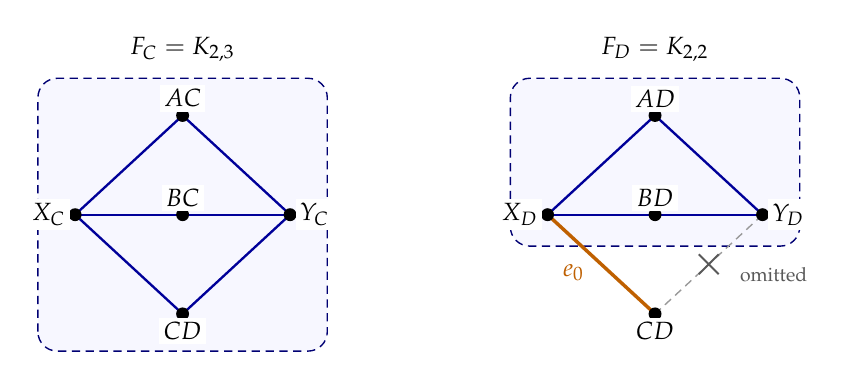
\begin{tikzpicture}[x=1.05cm,y=1.05cm,
  fan edge/.style={draw=blue!60!black,line width=.85pt},
  fan vertex/.style={circle,fill=black,inner sep=1.65pt},
  fan label/.style={font=\small,fill=white,inner sep=1.5pt},
  fan region/.style={rounded corners=7pt,draw=blue!45!black,
    densely dashed,fill=blue!3,line width=.5pt}]
  \begin{scope}[xshift=-3cm]
    \draw[fan region] (-1.75,-1.65) rectangle (1.75,1.65);
    \node[font=\small] at (0,2) {$F_C=K_{2,3}$};
    \coordinate (XC) at (-1.3,0);
    \coordinate (YC) at (1.3,0);
    \coordinate (Cac) at (0,1.2);
    \coordinate (Cbc) at (0,0);
    \coordinate (Ccd) at (0,-1.2);
    \foreach \L in {Cac,Cbc,Ccd}
      \draw[fan edge] (XC)--(\L)--(YC);
    \foreach \P in {XC,YC,Cac,Cbc,Ccd}
      \node[fan vertex] at (\P) {};
    \node[fan label,anchor=east] at (-1.36,0) {$X_C$};
    \node[fan label,anchor=west] at (1.36,0) {$Y_C$};
    \node[fan label,anchor=south] at (0,1.24) {$AC$};
    \node[fan label,anchor=south] at (0,.04) {$BC$};
    \node[fan label,anchor=north] at (0,-1.24) {$CD$};
  \end{scope}
  \begin{scope}[xshift=3cm]
    \draw[fan region] (-1.75,-.38) rectangle (1.75,1.65);
    \node[font=\small] at (0,2) {$F_D=K_{2,2}$};
    \coordinate (XD) at (-1.3,0);
    \coordinate (YD) at (1.3,0);
    \coordinate (Dad) at (0,1.2);
    \coordinate (Dbd) at (0,0);
    \coordinate (Dcd) at (0,-1.2);
    \foreach \L in {Dad,Dbd}
      \draw[fan edge] (XD)--(\L)--(YD);
    \draw[draw=orange!75!black,line width=1.25pt] (XD)--(Dcd);
    \draw[draw=black!40,densely dashed,line width=.5pt] (YD)--(Dcd);
    \draw[draw=black!65,line width=.7pt] (.53,-.48)--(.77,-.72)
                                              (.53,-.72)--(.77,-.48);
    \foreach \P in {XD,YD,Dad,Dbd,Dcd}
      \node[fan vertex] at (\P) {};
    \node[fan label,anchor=east] at (-1.36,0) {$X_D$};
    \node[fan label,anchor=west] at (1.36,0) {$Y_D$};
    \node[fan label,anchor=south] at (0,1.24) {$AD$};
    \node[fan label,anchor=south] at (0,.04) {$BD$};
    \node[fan label,anchor=north] at (0,-1.24) {$CD$};
    \node[fan label,text=orange!75!black,anchor=east] at (-.8,-.7) {$e_0$};
    \node[font=\scriptsize,anchor=west,text=black!65] at (.91,-.73) {omitted};
  \end{scope}
\end{tikzpicture}
\caption{A full fan and the exceptional fan.  The blue edges and their
endpoints form the indicated fans.  The loose edge
$e_0=X_D\text{--}CD$ belongs to $\Gamma$ but not to $F_D$; the crossed dashed
segment $Y_D\text{--}CD$ is absent from $\Gamma$.  In particular, $CD$ is
not a vertex of $F_D$.  The two occurrences of $CD$ denote the same line
vertex of $\Gamma$.}
\label{fig:fans}
\end{figure}


Choose an orientation for each edge once and for all. A \emph{field} is an edge position in a template or a position in a polygon word. An assignment gives one signed letter to each field. A walk reads that letter in the specified orientation and its inverse in the other orientation. The fields are bookkeeping coordinates; they all take values in the same alphabet.

A \emph{core hexagon} is the six-cycle obtained from three noncollinear points, the three lines joining them, and one representative over each point for which all six incidences are present. In particular, the all-$X$ choice is always permitted. Any three successive edges of a core hexagon contain at most two fields from each fan; the loose field, if present, belongs to no fan.

\FloatBarrier
\subsection{The independent tables}
For $n\ge1$, let
\[
 S_n=\{a_1,a_1^{-1},\ldots,a_n,a_n^{-1}\},\qquad N=2n.
\]
These are formal signed letters; assignments are not required to use distinct letters or to produce freely reduced words. Let
\begin{equation}\label{eq:model-parameters}
 f=2-\alpha,\qquad p=3-\beta,\qquad
 0<\alpha,\delta<1,\qquad 7\alpha<\beta<1.
\end{equation}
Additional smallness requirements will be imposed when we choose finitely many sampling tests.

\begin{definition}[The tables]\label{def:tables}
Use the following mutually independent Bernoulli arrays.
\begin{enumerate}[label=\textup{(\roman*)}]
\item For each point $i$, an array indexed by $S_n^{E(F_i)}$ includes every tuple with probability $N^{f-k_i}$. An included tuple, together with its type $i$, is a \emph{fan occurrence} $b$.
\item An array indexed by $S_n^{E(\Gamma)}$ marks every full core tuple with probability $N^{p-gf-1}$. A \emph{top occurrence} $a$ is a marked tuple whose restriction to every $F_i$ is an included fan occurrence. We write $a\to b$ when $b$ is the fan in one of the seven slots of $a$.
\item For each unoriented nonbacktracking two-edge path $\tau$ in $\Gamma$, choose one order and direction. Give $\tau$ a separate four-field array: its first two coordinates are the two core fields on $\tau$, and its last two are new coordinates. Include each row with probability $N^{-2-\delta}$. Its relator reads $\tau$, with the required orientation signs, followed by the two new letters around a closing path.
\item A separate six-field array includes each word in $S_n^6$ with probability $N^{-3-\delta}$. Its word is a relator.
\end{enumerate}
All included rows in \textup{(iii)} and \textup{(iv)} are imposed, not only rows matching some top occurrence. We call them \emph{decorations}; their lengths are $2h$, with $h\in\{2,3\}$.
\end{definition}

There is no ambiguity from opposite path directions: reversing one chosen convention simply inverts or reorders the corresponding coordinates, preserving the Bernoulli law. There are $90$ tables in Definition~\ref{def:tables}\textup{(iii)}. Indeed, the eleven point-representative vertices contribute $10\binom32+\binom22=31$ two-edge paths; the line degrees are $5,5,4,5,5,5,3$, contributing $59$ more.

The exponents in Definition~\ref{def:tables} are negative. In particular,
\[
 p-gf-1=-12-(\beta-7\alpha)<0.
\]
Each is therefore a valid probability. Distinct numerical tuples of a fixed table are independent. Top \emph{occurrences} are correlated because they may share fan slots; top \emph{marks} remain independent.

The expected counts explain the normalization of these probabilities.
For each fan type there are $N^{k_i}$ candidate tuples, so the expected
number of included fans is $N^f$. A fixed core tuple requires its mark
and seven independent fan entries. Since the fans contain $31$ fields
in total, the expected number of top occurrences is
\[
 N^{32}\,N^{p-7f-1}\prod_i N^{f-k_i}=N^p.
\]
Each square table has expected size $N^{2-\delta}$, and the six-letter
table has expected size $N^{3-\delta}$. Thus the expected exponents
are just below $2$ for fans and squares, and just below $3$ for tops
and hexagons. Section~\ref{sec:diagrams} explains how these deficits,
together with $\beta>7\alpha$, leave a positive margin in the diagram
estimates. The correlation between top occurrences is the
reason that their shared fan costs must be counted only once.

\subsection{The group and its two-complex}
The letter presentation has the generators $a_1,\ldots,a_n$. For each included fan and each top occurrence, impose the labels of all closed walks in its graph. Impose also the decoration words. This is a finite presentation: in each connected graph a fixed spanning tree supplies a finite basis of closed walks that suffices.

For the diagram arguments we use a specific finite two-dimensional CW complex $P$. Start with the letter bouquet, with vertex $o$. For each fan occurrence $b$ of type $i$, attach the cone on $F_i$ along its labelled map to the bouquet. The cone apex is a new vertex, also denoted $b$. For each vertex $v$ of $F_i$, its radial edge $r_{b,v}$ joins $b$ to the image $o$ of $v$. Every fan edge gives one triangle with one letter side and two radial sides. Different radial edges can have the same endpoints; they retain their distinct labels $v$.

The fan cones already fill all fan cycles. To impose the remaining
relations of a top occurrence $a$, take the ordinary Fano incidence
graph and subdivide the edge $D$--$CD$ once. Call the resulting graph
$B$. It has $15$ vertices and $22$ edges, hence cycle rank $8$,
matching the difference $15-7$ computed above. Map a point vertex $i$ to the apex
of the fan in slot $i$ of $a$, and map all line vertices and the
subdivision vertex to $o$. An ordinary incidence at $i$ maps to the
radial edge indexed by its line. The subdivided exceptional incidence maps to
\[
 r_{b_D,X_D}\quad\text{followed by the loose letter edge,}
\]
with the orientation giving the path from $X_D$ to $CD$. Attach the cone on this mapped graph, with its own new apex. We call its radial triangles \emph{top triangles}. Finally attach every decoration polygon. All these attachments are finite, and $P$ has dimension two.

\begin{lemma}[Presentation equivalence]\label{lem:model-presentation}
The complex $P$ has the fundamental group of the letter presentation above. In particular, it has a quotient isomorphic to $C_2$.
\end{lemma}
\begin{proof}
For a connected graph $H$ and a map $H\to X$ into a connected complex, attaching its cone changes $\pi_1X$ by the normal closure of the image of $\pi_1H$. It introduces no extra generator. This follows from van Kampen, or by choosing a spanning tree of $H$ and eliminating all but one of the new radial edges successively. The statement does not require distinct graph vertices to have distinct images.

It remains to check that the top macro graph imposes the required core relations after the fan relations. Each fan triangle replaces a fan edge by the two radial edges from its endpoints to the fan apex. A path in a fan can therefore be replaced, relative its endpoints, by the radial path through that apex. Apply these replacements to a closed core walk. Excursions through $X_i$ or $Y_i$ then cancel, leaving a closed walk in the mapped macro graph. At $D$, the only unreplaced edge is the loose edge; together with $r_{b_D,X_D}$ it gives exactly the exceptional subdivided incidence. Conversely, every macro turn can be replaced by a path in its connected fan. The two sets of relations have the same normal closure modulo the fan relations. This proves the presentation assertion.

The graph $\Gamma$, and each fan, is bipartite, so every closed-walk word has even length. The decorations have lengths four and six. Sending each original generator to the nonidentity element of $C_2$ respects all the defining relations and is surjective.
\end{proof}

\begin{remark}\label{rem:model-finite}
The cone description records occurrences, not just relator words. If the same fan occurs in several tops, its cone is attached only once. A top occurrence has its own cone, and a decoration occurrence has its own disk. These distinctions are essential in the multiplicity count of Section~\ref{sec:diagrams}.
\end{remark}

\subsection{The master pattern and admissible tests}
Define the finite \emph{master pattern} $\mathcal M$ by taking one top occurrence with its seven fan slots and, for each of the $90$ two-edge paths, one matching row of its square table. The two core coordinates of that row are identified with their core fields; its two closing coordinates are new. The separate six-letter array is not part of $\mathcal M$.

A \emph{match} is an assignment to the fields of $\mathcal M$ for which every required table entry is present, including the top mark. We denote the set of matches by $\Omega_n$. When it is nonempty, it carries its uniform probability measure. Its $32+2\cdot90$ fields include the shared core fields only once.

\begin{definition}[Admissible fields]\label{def:admissible}
A set of fields is \emph{admissible} if it is either
\begin{enumerate}[label=\textup{(\roman*)}]
\item a set of at most three distinct core fields containing at most two fields of each fan, or
\item a set of at most two fields of a single square decoration in $\mathcal M$.
\end{enumerate}
The loose core field does not count against any fan quota.
\end{definition}

The first case includes all three-edge half-paths of core hexagons. It also includes two $F_C$ fields together with the loose field, the combination that will produce the decisive midpoint identity. The second case includes every two-edge half-path in a decoration square.

Every match has a labelled realization of the core graph and the closing paths of its square decorations in the group: fix an anchor, and label a vertex by the word read along any path from the anchor. All closed-path labels are trivial by Lemma~\ref{lem:model-presentation} and the square relators. Consequently this group-valued vertex assignment is independent of the chosen path. For any action and basepoint, it gives a corresponding configuration of orbit points.

\section{Diagrams and linear filling}\label{sec:diagrams}

This section proves the combinatorial properties of the random complex
$P$ of Section~\ref{sec:model}.  An \emph{occurrence} means an included
tuple, together with its table type; copies of a cell in a diagram need
not be distinct occurrences.  All constants in this section may depend
on the fixed incidence template and on the fixed parameters, but not on
$n$.

\begin{theorem}\label{thm:diagram}
Fix sufficiently small positive $\alpha,\beta,\delta$ with
$\beta>7\alpha$, and put $f=2-\alpha$ and $p=3-\beta$.
As $n\longrightarrow\infty$, the probability tends to one that $P$ is
aspherical and its letter presentation satisfies a linear disk
isoperimetric inequality.
\end{theorem}

The central estimate will bound the number of faces in a bounded
piece of a normalized diagram by the number of its exposed sides. The expected
occurrence counts in Section~\ref{sec:model} have exponents
$2-\alpha$, $3-\beta$, and $h-\delta$ for fans, tops, and decorations
of length $2h$. The local incidence geometry compares these with the
values $2$, $3$, and $h$. After shared fan costs have been accounted
for, the differences $\alpha$, $\beta-7\alpha$, and $\delta$ supply the
strictly positive margin in the boundary estimate.

We first obtain a probability bound for every bounded collection of
distinct occurrences. We then normalize disk and sphere pictures so
that this bound also controls repeated copies of their cells. The
resulting estimate applies to arbitrary sets of faces, which lets us
partition a large picture by planar separators and sum the bounds on
its pieces. The same estimate proves linear filling for disks and
rules out nonzero two-cycles in the universal cover.

We retain every fan slot of a top occurrence when making a collection of
occurrences, even if a diagram uses only some of those slots.  This
convention is essential to the counting argument.

\subsection{Coincidence ranks}

Counting constraints while retaining repeated relator occurrences is
standard in random-group diagram arguments; see
Ollivier~\cite[Section~2]{Ollivier2004} and
Antoniuk--Friedgut--\L uczak~\cite[Section~3]{AntoniukFriedgutLuczak2017}.
We count the shared fan entries explicitly in the estimate below.

For a finite collection of top, fan, and decoration occurrences, its
\emph{field positions} are the following: the loose field of each top,
the $k_i$ fields of each fan occurrence of type $i$, and all fields of
each decoration occurrence.  A fan field is included only once when the
same fan occurrence occupies slots in several tops.  The
\emph{unsigned coincidence rank} $R$ is the number of positions minus
the number of distinct underlying generators represented at those
positions.  Thus a letter and its inverse have the same unsigned value.

\begin{lemma}\label{diagram:rank}
For each fixed integer $M$, with probability tending to one the
following holds simultaneously for every collection of at most $M$
distinct occurrences that contains all fan slots of its tops.  If the
collection has $s$ tops and $u$ fans, then
\begin{equation}\label{diagram:rank-bound}
 R\le (p-7f)s+fu+\sum_e(h_e-\delta),
\end{equation}
where the sum is over its decorations and $2h_e\in\{4,6\}$ is the
length of decoration $e$.
\end{lemma}

\begin{proof}
Fix the table types, the incidence of the fan slots, and a partition of
the field positions into unsigned-value classes.  There are only
finitely many such choices for fixed $M$.  Write $J$ for the number of
positions.  Assigning letters to a pattern of rank $R$ has at most
$C_M N^{J-R}$ possibilities: first choose one underlying generator per
class, then choose the signs of the positions.  The latter contributes
only a factor bounded in terms of $M$.

We count only choices whose occurrences are distinct within their
respective tables.  For such choices all the required Bernoulli trials
are independent.  Their product contributes the power of $N$ with
exponent
\[
 (p-7f-1)s+\sum_b(f-k_b)
       +\sum_e(h_e-\delta-2h_e).
\]
Here a shared fan occurrence appears once in the second sum, not once
per top using it.  Since
$J=s+\sum_b k_b+\sum_e2h_e$, the expected number of realizations of the
chosen pattern is at most
\[
 C_M N^{(p-7f)s+fu+\sum_e(h_e-\delta)-R}.
\]
If Equation~\eqref{diagram:rank-bound} fails, this exponent is negative.
There are finitely many exponents to consider for the fixed size bound,
so summing these expectations proves the assertion.
\end{proof}

\subsection{Spherical pictures and their reductions}

Lemma~\ref{diagram:rank} counts distinct occurrences, whereas a filling
diagram may use the same occurrence many times. We normalize the
diagram in two ways: the triangles incident to each top apex will be
grouped into polygons tracing simple macro cycles, and the cyclic
link at a fan apex will have no repeated radial label.
These properties will bound how often a field can appear near each
apex. For the asphericity argument, the normalization must also
preserve a prescribed lifted two-cycle.

An \emph{elementary picture} is a finite collection of oriented polygons with
orientation-reversing pairings of their sides, such that the resulting
closed oriented surfaces are spheres. Vertex links are taken to be
circles, with a separate source vertex for each link circle.
An interior face maps to a fan triangle, a triangle of a top cone, or a
decoration disk of $P$, with either orientation.  In the disk problem
there is one distinguished outside polygon whose boundary reads the
prescribed letter word; no extension of its interior to $P$ is required.
In the sphere problem there is no outside polygon.  Collapsed regions
mapping to vertices and free cancellations of edge paths have zero
face cost.  They can equivalently be recorded by thickening the paired
sides to strips and capping the boundary circles of the resulting
vertex regions.

Every cell has a specified map to $P$, including the index of each of
its sides.  Equal edge labels alone do not identify two side indices.
For a picture mapped to $\widetilde P$, its \emph{cellular chain} is the
sum of its signed lifted two-cells; the outside polygon is omitted.

\begin{lemma}\label{diagram:existence}
Every null letter word has a disk picture.  If
$c\ne0$ is a cellular two-cycle of $\widetilde P$, there is a finite
collection of spherical pictures with total cellular chain exactly
$c$.
\end{lemma}

\begin{proof}
The disk assertion is the cellular van Kampen construction, applied to
the finite cone and polygon complex.  Here is also a description that
applies to the sphere assertion.  Since $\widetilde P$ is simply
connected, the Hurewicz map
$\pi_2(\widetilde P)\longrightarrow H_2(\widetilde P;\mathbb Z)$ is an
isomorphism~\cite[Theorem~4.32]{Hatcher2002}.  There are no three-cells.
Consequently a sphere map
representing the class of $c$ has cellular two-chain equal to $c$, not
merely congruent to it modulo boundaries of three-cells.

Put this map in cellular general position.  One way to do so is to
choose an interior point in each two-cell, make its inverse image a
finite set of regular points, and take small disks about those
preimages.  Each such disk maps, with a sign, across that two-cell.
Retracting each punctured target cell to its boundary moves the
complement of these disks into the one-skeleton.  Inverse images of
interior edge points now give strips pairing the corresponding cell
sides; the remaining regions map to vertices.  Circular strips not
meeting cell sides may be cut and capped.  A vertex region with several
boundary components may likewise be replaced by a separate cap for
each component.  These operations are compressions along curves in an
oriented sphere.  They therefore produce a collection of oriented
spheres, not surfaces of positive genus.  They change none of the
signed cell disks or their lifts.  Components with no cell disks may
be discarded.  This gives the claimed spherical pictures and preserves
the chain $c$ exactly.

For a disk map, adjoin the distinguished outside polygon before the
same construction.  Keep that polygon as a single face throughout.
The construction preserves its word and gives one picture containing
it, possibly together with sphere components.  All the required
pictures are finite.
\end{proof}

At a vertex mapping to the apex of a top cone, every incident face is
a triangle of that cone.  Grouping its incident triangles gives a
polygon whose boundary is a closed walk in the macro graph of that top
occurrence.  We call it a \emph{top polygon}; its filling in $P$ is
always the indicated radial cone filling.  Its perimeter is the number
of these cone triangles.  The other interior faces remain fan triangles
and decoration disks.

The macro graph is the Fano incidence graph with one subdivided edge.
It has fifteen vertices.  A simple macro cycle has at most fifteen
sides, visits each point at most once, and visits at least three
points.  At a point it turns between two distinct \emph{ports}, namely
the radial labels of the fan there.  The ports are the incident line
vertices, except that the exceptional port at $D$ is $X_D$.

\begin{lemma}\label{diagram:normal-form}
A null letter word has a picture of minimum total top perimeter and,
subject to this, minimum number of remaining interior faces, with the
following properties.  The same assertion holds for a fixed nonzero
cellular two-cycle $c$, minimizing among finite collections of sphere
pictures whose total lifted cellular chain is exactly $c$.
\begin{enumerate}
\item Every top polygon is a simple macro cycle.
\item Adjacent top polygons do not use the same side of the same
top occurrence.  Two copies of one fan triangle cannot be adjacent
along equally indexed sides, and two copies of one decoration cannot
be adjacent along the same position of that decoration.
\item At each fan-apex instance, the cyclic list of radial labels has
no repetition.  A circuit with two distinct parallel steps is
permitted.  Each such circuit has at most five steps.  If it contains
no top turn, it has at least four fan triangles.
\end{enumerate}
The modifications establishing these properties preserve the outside
word and, in the sphere problem, the exact lifted cellular chain.
\end{lemma}

\begin{proof}
The nonempty class of finite pictures in
Lemma~\ref{diagram:existence} has a lexicographic minimum for the stated
pair of nonnegative integer costs.  In the sphere case fix the chain
$c$ once and for all in taking this minimum.

\emph{Simple macro cycles.}  Consider a top polygon whose macro walk repeats a template
vertex.  Its two boundary points at that repetition have the same
lifted value: both are joined to the same lifted top apex by the same
indexed cone spoke.  Split the polygon by a chord collapsed to that
vertex.  The two resulting macro walks have the same total perimeter
and the same total cone chain.  A free backtrack cancels two oppositely
oriented copies of a single lifted cone triangle and reduces total
perimeter by two.  Delete any resulting empty polygons.  Repeating
splitting and removal of backtracks therefore gives simple macro
cycles.  Collapsed chords may be put in
the picture form of Lemma~\ref{diagram:existence}; they carry no
two-chain.  This proves the first property.

\emph{Cancellation.}  Suppose two top polygons meet at the same
macro side of one occurrence.  The two elementary cone triangles
incident to that side are copies of the same triangle with opposite
orientations.  Their lifts agree, because the common lifted macro side
determines the lifted triangle and its apex.  Cancel the pair and
merge the remaining cone walks.  This reduces total top perimeter by
two.  It is an ordinary diagram cancellation: one uses the two face
interiors and a thin strip across the specified common side, so other
contacts between their boundaries cause no obstruction.  Any vertex
regions produced by the cancellation are capped as above.  A
same-template contact cannot occur between two sides of a single
simple top polygon, because a simple macro cycle uses each edge at
most once.  The identical cancellation of two fan triangles or two
decoration disks along equally indexed sides reduces the second cost
without increasing the first.  These cancellations preserve the
cellular chain, so they are forbidden by minimality in both problems.

\emph{Fan-apex links.}  Fix a source vertex $v$
mapping to a fan apex $b$.  A step in its link is either a fan triangle
or a corner of a top polygon.  Suppose two different outgoing spokes
at $v$ have the same radial label.  Each spoke is an edge from $v$ to a
vertex mapping to the letter-bouquet vertex.  Cut the side pairings of
these two edges and pair them crosswise, with the outgoing orientations
at $v$ agreeing.  This preserves the orientation of every face and all
face maps.  In terms of vertex-link cycles, it splits the link cycle of
$v$ into two.  At the far ends it either merges two distinct vertex
cycles or splits one vertex cycle.

For completeness, this switch preserves the genus-zero condition.
The numbers of faces and edges do not change.  When the two far
vertices were distinct, the total vertex count does not change, and
the affected surface remains connected: both switched edges are
incident to the merged far vertex.  When the far vertices were the
same, the total vertex count increases by two. There can be at most
two affected components after either switch. To see this, cut the two
corresponding edges of the connected dual graph before re-pairing
their four exposed half-edges. Every component of the cut graph
contains an exposed half-edge: otherwise it was already disconnected
before the cut. After re-pairing, every component therefore contains
one of the two switched edges. This argument includes loops and
parallel edges in the dual graph.
In the first case the connected oriented surface consequently has
Euler characteristic two.  In the second case the total Euler
characteristic is four, which forces exactly two oriented spheres.
All unaffected spheres are retained, and the outside polygon remains
one unchanged face.

The switch is also valid for the fixed lifted chain.  The repeated
radial label and the lifted initial fan vertex determine the same
lifted radial edge and far endpoint.  Thus the new vertex
identifications agree in $\widetilde P$, and every lifted face is
unchanged.  Each switch increases the number of fan-apex instances
while keeping the finite set of polygon corners fixed.  Repetition
therefore terminates.  The two minimized costs are unchanged, so a
newly created forbidden adjacency would still contradict their
minimality by the cancellation just described.

The resulting link uses each radial label at most once.  There are at
most five labels in any fan.  A two-step link made only of fan
triangles is the reverse traversal of one edge of the simple fan graph;
the two triangles would cancel along an equally indexed radial side.
Every other nonempty triangle-only link is a circuit in the simple
bipartite fan graph and has length at least four.  This proves the last
property.
\end{proof}

The outside word uses only letter edges, so an outside polygon never
meets a fan-apex instance.  In particular each full link considered in
Lemma~\ref{diagram:normal-form} is a cyclic link of interior faces.

\subsection{Weights on a bounded fragment}

Fix a normal picture.  A \emph{fragment} is any selection of its
interior faces; the selection need not be connected or simply
connected.  Keep a pairing of sides precisely when both incident faces
are selected.  All other selected sides are fragment boundary sides.
Let $T,Q,E$ be the numbers of selected top polygons, fan triangles, and
decoration disks, respectively, and put $A=T+Q+E$.

For a top occurrence $a$ let $t_a$ be its number of selected top
polygons, and for a decoration occurrence $e$ let $t_e$ be its selected
multiplicity.  At a fan-apex instance $z$ represented in the fragment,
let $d_z$ count selected top turns and $q_z$ count selected fan
triangles.  It is \emph{partial} if not every step of its full cyclic
link is selected.

For a fan occurrence $b$, two multiplicities must be distinguished.
The number of represented apex instances bounds the actual use of
each fan field. We must also retain this fan whenever we retain a top
of sufficiently large multiplicity that requires it. The fan weight
must therefore dominate the largest such top multiplicity. Write
\[
 r_b=\#\{z:z\text{ is represented over }b\},\qquad
 m_b=\max_{a\to b}t_a,\qquad
 S_b=\sum_{a\to b}t_a,\qquad
 w_b=\max\{r_b,m_b\}.
\]
Empty maxima are zero.  All fan slots of every selected top are
included in these definitions, whether or not a polygon of that top
visits the fan.  In particular
\begin{equation}\label{diagram:slot-sum}
 \sum_b S_b=7T.
\end{equation}
Write $J_b$ for the number of partial instances over $b$, and let
$P_b^*$ count the selected loose top sides belonging to turns at this
fan.  This number is zero unless $b$ has type $D$.  Each such loose side
records one incidence with the exceptional radial port $X_D$.

Let $I$ count internal contacts between two letter sides of the
fragment.  Radial side contacts are not counted in $I$.  Denote the
numbers of letter and radial fragment boundary sides by $B_{\rm raw}$
and $B_{\rm rad}$, and put $B=B_{\rm raw}+B_{\rm rad}$.

We first use the coincidence bound to control internal letter contacts.
The remaining estimate is local at fan apices: full links contribute
no error, while partial links contribute an error paid by radial
boundary sides.  Combining the two estimates will bound the fragment's
area by its total boundary length.

\begin{lemma}\label{diagram:weighted-rank}
Suppose Equation~\eqref{diagram:rank-bound} holds for collections of at
most $8A$ occurrences.  Then
\begin{equation}\label{diagram:contact-bound}
 I\le pT+f\sum_b(w_b-S_b)
              +\sum_e(h_e-\delta)t_e.
\end{equation}
\end{lemma}

\begin{proof}
Give each fan field of $b$ weight $w_b$, each loose field of $a$ weight
$t_a$, and each field of a decoration $e$ weight $t_e$.  These are
upper bounds for their side multiplicities in the fragment.  Indeed a
fan field is used at most once at a given normalized fan-apex link, so
its multiplicity is at most $r_b$.  A simple top polygon uses its loose
field at most once, and a copy of a decoration uses each indexed field
once.

For each integer $j\ge1$, apply
Equation~\eqref{diagram:rank-bound} to the positions of weight at least
$j$.  This is an eligible collection: $t_a\ge j$ implies
$w_b\ge m_b\ge t_a\ge j$ for every slot $a\to b$.  Its size is at most
$8A$, since there are at most $T$ distinct tops, at most $7T+Q$ fans,
and at most $E$ decorations.  Sum the resulting inequalities over $j$.
Within an unsigned-value class, the sum of its ranks is its total
weight minus its largest position weight.  Thus, writing
$\mathcal C$ for the unsigned-value classes, we obtain
\begin{equation}\label{diagram:weighted-coincidence}
 \sum_{C\in\mathcal C}
 \left(\sum_{v\in C}\operatorname{wt}(v)
                  -\max_{v\in C}\operatorname{wt}(v)\right)
 \le (p-7f)T+f\sum_b w_b+\sum_e(h_e-\delta)t_e.
\end{equation}

Every internal letter contact joins two different field positions.
For fan triangles and decorations this follows from the cancellations
in Lemma~\ref{diagram:normal-form}; for two loose top sides it follows
from the same-occurrence top cancellation.  A contact between different
kinds of cells automatically has different positions.  In each class
$C$, choose one maximum-weight position.  Charge each internal contact
to one of its endpoints other than that position.  Such an endpoint
always exists.  Different contacts use different actual side copies,
so the charge to any position is at most its side multiplicity and
hence at most its weight.  This proves that $I$ is bounded by the left
side of Equation~\eqref{diagram:weighted-coincidence}.  Using
Equation~\eqref{diagram:slot-sum} on its right side gives
Equation~\eqref{diagram:contact-bound}.
\end{proof}

This argument allows arbitrary cycles and repetitions in the contact
graph.  It charges side copies, and does not require the contacts to
form a forest.

\begin{lemma}\label{diagram:apex}
For every fan occurrence $b$ in a fragment,
\begin{equation}\label{diagram:apex-bound}
 \sum_{z\mapsto b}d_z+2(w_b-S_b)
 \le \frac12\left(\sum_{z\mapsto b}q_z+P_b^*\right)+2J_b.
\end{equation}
Moreover
\begin{equation}\label{diagram:partial-bound}
 2\sum_bJ_b\le B_{\rm rad}.
\end{equation}
\end{lemma}

\begin{proof}
First suppose $w_b=r_b$.  A simple top polygon has at most one turn at
this fan, so $S_b\ge\sum_{z\mapsto b}d_z$.  Consequently the left side
of Equation~\eqref{diagram:apex-bound} is at most
$\sum_{z\mapsto b}(2-d_z)$.
For a full link with $d_z=0$, at least four fan triangles give the
required inequality.  For a full link with $d_z=1$, the triangles form
a path in the fan between the two distinct ports of that top turn.
Ordinary ports are distinct line vertices, so this path has at least
two edges.  The only exception is a path incident to the port $X_D$;
it may have one edge, in which case its top turn has the loose side
counted by $P_b^*$.  Thus in either case its triangle count plus its
loose-side payment is at least two.  For $d_z\ge2$ the expression
$2-d_z$ is nonpositive.  At a represented partial link with $d_z=0$
there is at least one selected fan triangle, so its deficit is at most
$3/2$.  With $d_z=1$ its deficit is at most one, and with $d_z\ge2$
it is nonpositive.  Thus the error $2J_b$ suffices in this case.

Now suppose $w_b=m_b>r_b$, and choose a top occurrence $a_0$ with
$t_{a_0}=m_b$.  Call its turns dominant.  Let $x$ and $y$ be the total
numbers of selected dominant and nondominant turns over $b$.
Nondominant selected faces have at most one turn each at this fan,
including when other selected faces omit the fan entirely; hence
$y\le S_b-m_b$.  It follows that
\begin{equation}\label{diagram:dominant-algebra}
 \sum_{z\mapsto b}d_z+2(m_b-S_b)
       =x+y-2(S_b-m_b)\le x-y.
\end{equation}

Consider a full link.  In its cyclic list of turns the number of
consecutive dominant-to-dominant interfaces is at least the number of
dominant turns minus the number of other turns.  To see this, assign to
each dominant turn its following turn: at most as many dominant turns
can be followed by a nondominant one as there are nondominant turns.
A single turn is followed by itself.  Between a counted pair of turns
there is a path of fan triangles.  This path cannot have length zero,
because then the two top polygons use the same radial side of the
same occurrence $a_0$, forbidden by
Lemma~\ref{diagram:normal-form}.  If the path has length one, it must
have an exceptional port, since the other ports lie in the line part
of the bipartite fan graph.  That port has its loose-side payment.
Thus the path length plus the available payments is at least two for
each counted interface.  The triangle paths are disjoint portions of
the link.  A port incidence is an endpoint of just one such intervening
path, so no loose-side payment is used twice.  The triangle counts and
payments at full links therefore bound twice their total
dominant-minus-nondominant count from below.

At a partial link, the selected steps form a nonempty proper subset
of a cyclic list of at most five steps.  Split this subset into maximal
consecutive selected runs.  Each run and each intervening unselected
gap contains a step, so there are at most two runs.  In a run containing
turns, let $k$ and $l$ be the numbers of dominant and nondominant turns.
Their linear turn list has at most $l+1$ blocks of dominant turns.
Consequently, if $H$ counts its consecutive dominant-to-dominant
interfaces, then
\[
 H\ge k-l-1,\qquad k-l\le H+1.
\]
The fan-triangle path at each of these interfaces is entirely selected.
The same indexed-side cancellation and exceptional-port argument used
for a full link shows that its length plus its available loose-side
payments is at least two.  Different interfaces, including those in
different runs, use disjoint triangle paths and distinct port incidences,
so no payment is used twice.  A run without turns contributes zero to
the dominant-minus-nondominant count.  Summing over the at most two runs
therefore bounds that count by half the selected triangle count and
loose-side payments, plus two.

Choose the dominant occurrence $a_0$ once for the entire fan occurrence
$b$, and apply these estimates separately at all its apex instances.
They do not require the fragment to be connected, or every selected
polygon of $a_0$ to visit this fan.  Summing the partial- and full-link
estimates, and then using
Equation~\eqref{diagram:dominant-algebra}, proves
Equation~\eqref{diagram:apex-bound} also in the second case.

Finally, a represented partial cyclic link has at least two
transitions between selected and unselected steps.  Each transition
is a radial edge with exactly one selected incident face, and hence
is a radial fragment boundary side.  A radial side belongs to only one
fan-apex instance.  This proves
Equation~\eqref{diagram:partial-bound}.
\end{proof}

\begin{lemma}\label{diagram:fragment}
Put
\begin{equation}\label{diagram:kappa}
 \kappa=\min\{\beta-7\alpha,\alpha/5,\delta\}>0.
\end{equation}
If Equation~\eqref{diagram:rank-bound} holds for collections of at most
$8A$ occurrences, then every fragment of area $A$ satisfies
\begin{equation}\label{diagram:fragment-bound}
 A\le C_0 B,\qquad C_0=\frac{1}{\kappa}.
\end{equation}
\end{lemma}

\begin{proof}
Write $W=\sum_b w_b$ and $P^*=\sum_bP_b^*$.  Every simple top polygon
has at least three turns.  Summing
Equation~\eqref{diagram:apex-bound}, and using
Equation~\eqref{diagram:slot-sum}, gives
\begin{equation}\label{diagram:nominal-apex}
 3T+2(W-7T)\le \frac{Q+P^*}{2}+2\sum_bJ_b.
\end{equation}
The right side of Equation~\eqref{diagram:contact-bound} can be written
as
\[
 3T+2(W-7T)+\sum_eh_et_e-\Delta,
 \qquad
 \Delta=(\beta-7\alpha)T+\alpha W+\delta E.
\]
There are at most five selected triangles at a represented fan-apex
instance, so
$Q\le5\sum_b r_b\le5W$.  Therefore
\begin{equation}\label{diagram:defect}
 \Delta\ge\kappa(T+Q+E)=\kappa A.
\end{equation}
The total number of raw side copies in the fragment is
\[
 R_{\rm raw}=Q+P^*+\sum_e2h_et_e.
\]
Equations~\eqref{diagram:contact-bound} and
\eqref{diagram:nominal-apex} imply
\[
 I\le \frac{R_{\rm raw}}2-\Delta+2\sum_bJ_b.
\]
Since $B_{\rm raw}=R_{\rm raw}-2I$,
Equations~\eqref{diagram:partial-bound} and
\eqref{diagram:defect} give
\[
 2\kappa A\le 2\Delta
       \le B_{\rm raw}+4\sum_bJ_b
       \le B_{\rm raw}+2B_{\rm rad}\le2B.
\]
This is Equation~\eqref{diagram:fragment-bound}.
\end{proof}

\subsection{From bounded fragments to all pictures}

The probability estimate controls only bounded collections of
occurrences. To use it for an arbitrarily large picture, we partition
the faces into bounded sets while cutting few contacts. A fragment
was allowed to be disconnected and to have holes, so any partition
of the dual graph gives eligible fragments. The following separator
estimate makes their total new boundary small enough to absorb into
the area bound.

\begin{lemma}\label{diagram:separator}
For every $D<\infty$ and $\eta>0$ there is an integer $K=K(D,\eta)$
such that the vertices of any finite planar multigraph of maximum
degree at most $D$ can be partitioned into sets of size at most $K$,
with at most $\eta$ times the total number of vertices edges crossing
between sets.
\end{lemma}

\begin{proof}
Ignore loops and apply the planar separator theorem to the underlying
simple graph.  In a graph with $q$ vertices it gives a set of at most
$c\sqrt q$ vertices whose removal leaves two sets, with no edges
between them, each of size at most $2q/3$; one may take
$c=2\sqrt2$ \cite[Corollary~2]{LiptonTarjan1979}.  Repeat inside every set larger
than $K$, and make every removed separator vertex a singleton part.

Charge $c/\sqrt q$ to every vertex present in a recursive set of size
$q$.  These charges pay for all removed separator vertices.  For any
fixed original vertex, the successive set sizes containing it decrease
by a factor at most $2/3$ while they exceed $K$.  Reading that sequence
backward shows that its total charge is at most
\[
 \frac{c}{\sqrt K}\sum_{j\ge0}(\sqrt{2/3})^j
       =\frac{c}{(1-\sqrt{2/3})\sqrt K}.
\]
If the original graph has $A$ vertices, the number of removed
separator vertices is at most $C A/\sqrt K$, where
$C=c/(1-\sqrt{2/3})$.  Every edge crossing between final parts has a
removed separator vertex as an endpoint.  The degree bound therefore
limits their number, counting multiplicity, to $DC A/\sqrt K$.
Choose $K$ so large that $DC/\sqrt K\le\eta$.  Disconnected graphs
are treated component by component.
\end{proof}

\begin{proof}[Proof of Theorem~\ref{thm:diagram}]
Fix the parameters, so that $\kappa$ and $C_0$ in
Lemma~\ref{diagram:fragment} are positive constants.  Choose
$\eta>0$ with $2C_0\eta\le1/2$, and apply
Lemma~\ref{diagram:separator} with $D=15$.  This gives a fixed finite
threshold $K$.  By Lemma~\ref{diagram:rank}, with probability tending
to one Equation~\eqref{diagram:rank-bound} holds for all collections of
at most $8K$ occurrences.  Work with any realization having that
property.  The remainder of the proof is deterministic and applies
simultaneously to every picture for this realization.

For a normal picture, the dual graph of its interior faces and their
contacts is planar of degree at most fifteen.  Fan triangles have
three sides, decorations have at most six, and simple top polygons
have at most fifteen.  Parallel contacts and self-contacts cause no
problem in Lemma~\ref{diagram:separator}.  Partition its $A$ interior
faces into fragments of size at most $K$, cutting at most $\eta A$
contacts.  Let $B_0$ count contacts with the outside polygon; in the
sphere problem set $B_0=0$.  The sum of fragment boundary lengths is
at most $B_0+2\eta A$.  Lemma~\ref{diagram:fragment} applies to every
fragment, and summing it gives
\[
 A\le C_0(B_0+2\eta A),
 \qquad\text{hence}\qquad A\le2C_0 B_0.
\]
In a disk picture whose outside word has length $\ell$, one has
$B_0\le\ell$; outside-to-outside pairings represent free boundary
cancellations and do not add an interior contact.  Thus the normal
picture uses at most $2C_0\ell$ interior faces.

If a nonzero cellular two-cycle $c$ existed in $\widetilde P$, use its
normal spherical picture supplied by
Lemmas~\ref{diagram:existence} and \ref{diagram:normal-form}.
For it $B_0=0$, forcing $A=0$.  Its cellular chain would then be zero,
contrary to its construction.  Therefore
$H_2(\widetilde P;\mathbb Z)=0$.  The universal cover is a simply
connected two-dimensional CW complex, so all its reduced homology
groups vanish.  If it had a first nonzero homotopy group, the
Hurewicz theorem would identify it with a nonzero homology
group~\cite[Theorem~4.32]{Hatcher2002}.
It is consequently weakly contractible, and the Whitehead theorem
makes it contractible~\cite[Theorem~4.5]{Hatcher2002}.
This proves asphericity.

We finish by making explicit the claimed filling inequality over
letters.  Choose a vertex of every fan template and, for each of its
vertices, a fixed path from the chosen vertex to that vertex.  These
paths have length at most two.  Send every fan-apex vertex of a normal
picture to the bouquet vertex, and replace its indexed radial edge by
the label word of the corresponding fixed fan path, with the
appropriate orientation.  A fan triangle boundary becomes a closed
walk in that fan of length at most five.  A top polygon boundary
becomes a closed walk in its copy of $\Gamma$: at an ordinary point,
its two radial paths concatenate to a fan path between the two ports;
at the exceptional point the path to $X_D$ is followed by the loose
edge.  Its expanded length is at most thirty.  A decoration boundary
is unchanged.

Use as a finite letter presentation all simple cycle relators in each
included fan and top graph, together with the decoration rows.  This
presents the same group by the cone construction in
Section~\ref{sec:model}.  Any closed graph walk of length at most
thirty splits at repeated vertices into at most thirty simple cycles,
after free backtracks are erased.  Each expanded face above thus has
a filling with at most thirty relator disks in this presentation.
Replacing the faces of the normal picture by these fillings leaves
the outside letter word unchanged and produces a disk diagram, with
free folds allowed, of area at most
$60C_0\ell$.  Sphere components can be discarded.  Any other fixed
finite choice of defining cycle relators gives the same linear
inequality after bounded relator substitutions.  This proves the
theorem.
\end{proof}

\begin{remark}\label{diagram:quantifiers}
The separator threshold is chosen after the positive parameters are
fixed and before $n$ tends to infinity.  No uniform bound as
$\alpha,\beta,\delta\longrightarrow0$ is asserted or required.
For each fixed parameter choice, the single finite-collection event in
Lemma~\ref{diagram:rank} controls all disk words and all cellular
two-cycles simultaneously.
\end{remark}

\section{Conditional sampling from the nested tables}\label{sec:sampling}

The relations will be tested against an action chosen after all the tables
have been sampled.  We therefore prove statements about total variation of
finite distributions on table matches.  These statements do not refer to a
target metric space.  In particular, they will apply simultaneously to all
uniformly bounded functions on the relevant assignments, including functions obtained
from a subsequently chosen action.

\subsection{The master pattern and its critical exponents}

Recall the master pattern $\mathcal M$ from Section~\ref{sec:model},
and let $\mathcal F$ be its field set.  Its required entries are the
seven fan entries, the top-mark entry, and one entry from each of the
$90$ four-letter tables.  In each four-letter entry its first two fields are
identified with the corresponding core fields; its other two fields are
new and are used in no other entry.  The six-letter table is not part of
$\mathcal M$.  Thus $|\mathcal F|=212$.  Write $\mathcal R$ for the set of
its $98$ array entries and $E_\rho\subseteq\mathcal F$ for the field
support of $\rho\in\mathcal R$.  Each $\rho$ belongs to a different
Bernoulli array.  The order of its coordinates is fixed throughout.

A \emph{match} is a map $\sigma:\mathcal F\to S_n$ for which every
required array entry is present.  No injectivity is required of a single
match.  We write $\Omega_n$ for the random set of matches and, when it is
nonempty, write $\mu_N$ for its uniform probability measure.

Recall from Definition~\ref{def:admissible} that a set of fields is
admissible if it consists either of at most three core fields, at most
two in each fan, or of at most two fields of one square decoration.
The loose field belongs to no fan.
\begin{definition}\label{sample:def-test}
A \emph{conditional test} is a triple $(I,e,t)$ with
$I\subseteq\mathcal F$, $e\in\mathcal F\setminus I$,
$I\cup\{e\}$ admissible, and $t$ a positive integer.
\end{definition}

For $\theta=(\alpha,\beta,\delta)$ define $c_\rho(\theta)$ so that
the inclusion probability of entry $\rho$ is $N^{-c_\rho(\theta)}$.
Its value and its critical value $c_\rho=c_\rho(0)$ are
\begin{equation}\label{sample:eq-costs}
\begin{array}{c|c|c}
\text{entry}&c_\rho(\theta)&c_\rho\\ \hline
\text{fan }i&k_i-2+\alpha&k_i-2\\
\text{top mark}&12+\beta-7\alpha&12\\
\text{four-letter entry}&2+\delta&2.
\end{array}
\end{equation}
For a set of fields $W$ put
\begin{equation}\label{sample:eq-h}
h_\theta(W)=|W|-\sum_{\rho:E_\rho\subseteq W}c_\rho(\theta),
\qquad h(W)=h_0(W).
\end{equation}
Thus $N^{h_\theta(W)}$ is the expected number of assignments to $W$
for which all required entries supported in $W$ are present.
The function $h$ is submodular.  Indeed, for each fixed $E_\rho$,
the indicator of $E_\rho\subseteq W$ is supermodular, and all
$c_\rho$ are nonnegative.  Notice also that
\begin{equation}\label{sample:eq-master-mean}
h(\mathcal F)=212-(17+12+180)=3,
\qquad
\E|\Omega_n|=N^{h_\theta(\mathcal F)}
             =N^{3-\beta-90\delta}.
\end{equation}
The expectation is exact: each assignment uses one entry from each of
the distinct arrays, so all of its inclusion requirements are independent.

\begin{lemma}\label{sample:lem-budget}
For every $W\subseteq\mathcal F$,
\begin{equation}\label{sample:eq-budget}
h(W)\geq\min\{2,|W|\}.
\end{equation}
If $S$ is admissible and $S\subseteq W$, then
\begin{equation}\label{sample:eq-admissible-budget}
h(W)\geq |S|.
\end{equation}
\end{lemma}
\begin{proof}
First consider only the core part of $W$.  Let $a_i$ be its number of
fields in $F_i$, and let $\ell\in\{0,1\}$ indicate the loose field.
Before charging the top mark, the exponent is
\[
\sum_i\bigl(a_i-(k_i-2)\mathbf 1_{\{a_i=k_i\}}\bigr)+\ell
\ \geq\ \sum_i\min\{a_i,2\}+\ell.
\]
The top-mark cost is charged only for the complete core.  For that set
the exponent is $32-17-12=3$.  Consequently every core subset has
exponent at least the size of any admissible core subset it contains,
and at least the smaller of two and its own cardinality.

Now add the fresh fields of the four-letter entries.  Adding one fresh
field of an entry adds one to the exponent.  Adding both adds two and
can charge the cost two only if that entry's two core fields are also
present.  The net contribution of each pair of fresh fields is therefore
nonnegative.  This proves Equation~\eqref{sample:eq-admissible-budget}
when $S$ consists of core fields, and proves
Equation~\eqref{sample:eq-budget} when $W$ has at least two core fields.
If $W$ has fewer than two core fields, no four-letter entry is charged,
and no fan or top entry is charged either.  In that case $h(W)=|W|$.
This proves Equation~\eqref{sample:eq-budget} in all cases.  Finally,
an admissible subset of one four-letter entry has size at most two, so
its required bound follows from Equation~\eqref{sample:eq-budget}.
\end{proof}

Fix a conditional test $(I,e,t)$.  To couple $t$ matches agreeing on
$I$, we will require them to agree on a possibly larger set $U$.
The purpose of this enlargement is to make every further extension
increase the critical exponent.  For example, if $I$ consists of two
fields in one fan $F_i$, then completing that fan leaves the exponent
unchanged:
\[
h(I)=2=h(E(F_i)).
\]
Once the fan fields have been included, adjoining both fresh fields of
any square whose two core fields lie in that fan also leaves the exponent
unchanged.  These are examples of the enlargements that the choice of
$U$ must absorb.

In general, $|I|\leq2$, and every entry support has at least three
fields, so $h(I)=|I|$.  Choose an inclusion-maximal set
$U\supseteq I$ such that
\begin{equation}\label{sample:eq-closure}
h(U)=|I|.
\end{equation}
Such a set exists because the field set is finite.  The next two
properties are the reason for this choice:
\begin{equation}\label{sample:eq-closure-gap}
e\notin U,
\qquad
h(U\cup V)-h(U)\geq1
\quad\text{for every nonempty }V\subseteq\mathcal F\setminus U.
\end{equation}
The first follows from Equation~\eqref{sample:eq-admissible-budget}
applied to $I\cup\{e\}$.  For the second, every superset of $U$
has exponent at least $|I|$ by the same lemma applied to $I$.
Maximality rules out equality for a strict superset, and all critical
exponents are integers.

\subsection{Stars and their overlap estimates}

Form a star $\mathcal M_U^{(t)}$ from $t$ ordered copies of
$\mathcal M$ by identifying all copies of each field in $U$.
Entries supported entirely in $U$ are also identified.  Each other
entry retains one copy in each branch.  We require assignments to this
star to be \emph{injective in each field}: for each
$s\in\mathcal F\setminus U$, its $t$ branch values must be pairwise
distinct.  Values in different fields may coincide.  All fields continue
to take values in the same alphabet $S_n$.

This injectivity has two consequences.  First, copies of an entry not
supported in $U$ are distinct tuples in their array, since some one of
their coordinates lies outside $U$.  Second, when one branch is fixed,
an entry in another branch that is not supported in $U$ cannot equal
the corresponding entry of the fixed branch.  Thus all random variables
counted below are products of distinct Bernoulli trials, after explicitly
removing any trials on which we have conditioned.

We give the overlap count in detail because the coordinates are not
disjoint letter domains.  An \emph{overlap type} between two star
assignments specifies precisely which entries of each array coincide
across the two stars.  There are finitely many such types for fixed $t$.
Each equality of array entries equates corresponding coordinates.  For
a given field $s\notin U$, injectivity implies that these equalities
give a partial matching between the $t$ branch variables of the first
star and those of the second.  Different arrays may use different
partial matchings; their union must still be a partial matching whenever
the overlap type is realizable.  Otherwise two different branch values
of the same field would be forced equal.  For $s\in U$ there is just
one variable in each star.  In particular, an equality never compares
two different coordinate fields, even if their numerical letter values
happen to be equal.

Here is the resulting counting rule.  Reveal the first assignment.
Suppose the equalities of an overlap type prescribe the values of $q$
distinct, previously unpinned variables in the second assignment.
For each field with unpinned variables, there are a bounded number of
those variables, and they are chosen uniformly without replacement,
possibly avoiding one already pinned value.  A field whose variables
are all pinned contributes a factor one.  Prescribing $q_s$ of them has probability at most
$C_t N^{-q_s}$: the number of remaining choices is at most
$N^{r-q_s}$, whereas the number of unrestricted choices is a falling
factorial $(N-a)_r$, with $r\leq t$ and $a\in\{0,1\}$.
Multiplying over the finitely many fields gives
\begin{equation}\label{sample:eq-assignment-penalty}
\text{fraction of pairs having the specified overlap}
\ \leq\ C_tN^{-q}.
\end{equation}
Incompatible specifications simply contribute zero.

If the coincident, unconditioned entries have total actual cost $C$,
their joint inclusion probability divided by the product of the two
individual inclusion probabilities is $N^C$.  All other trials are
independent.  Consequently this overlap type contributes at most
\begin{equation}\label{sample:eq-variance-rule}
C_t N^{-q+C}
\end{equation}
to the relative variance of the count in question.  Pairs with no
coincident unconditioned entry have covariance zero, including when
they have coincident values that do not complete any common entry.
To justify the relative-variance normalization directly, all candidate
assignments in any one of our counting problems have the same
probability of inclusion, and Equation~\eqref{sample:eq-assignment-penalty}
bounds the fraction of pairs of such candidates.  Summing their
covariances and dividing by the square of the expectation gives
Equation~\eqref{sample:eq-variance-rule}, summed over the finitely many
nonempty overlap types.

We first apply this rule to a single copy of $\mathcal M$.  If $W$ is
the set of fields belonging to its shared entries, then $q=|W|$ and
the recovered cost is at most the sum of the costs of all entries
supported in $W$.  Its critical excess is therefore at least
$h(W)>0$.  For sufficiently small actual parameters, every one of
these finitely many positive excesses stays positive.  It follows that
\begin{equation}\label{sample:eq-single-concentration}
\frac{\operatorname{Var}|\Omega_n|}{(\E|\Omega_n|)^2}=o(1).
\end{equation}
In particular the master count is asymptotic to its expectation in
probability.  We always choose the parameters small enough that the
exponent in Equation~\eqref{sample:eq-master-mean} is positive.

For the two star counts, write
\[
C_U(\theta)=\sum_{\rho:E_\rho\subseteq U}c_\rho(\theta),
\qquad
C_{\mathrm{out}}(\theta)
 =\sum_{\rho:E_\rho\not\subseteq U}c_\rho(\theta),
\qquad d=|\mathcal F\setminus U|.
\]
Let $Z_N$ be the number of present injective stars.  With
$(N)_t=N(N-1)\cdots(N-t+1)$,
\begin{equation}\label{sample:eq-star-mean}
\E Z_N
 =N^{|U|}(N)_t^d
  N^{-C_U(\theta)-tC_{\mathrm{out}}(\theta)}.
\end{equation}

\begin{lemma}\label{sample:lem-conditional-counts}
For each fixed conditional test, sufficiently small actual parameters
have the following properties as $N\to\infty$.
\begin{enumerate}
\item Fix any assignment $\sigma:\mathcal F\to S_n$, place it in a
specified branch, and condition on it being a match.  Let $A_\sigma$
count its extensions to a present injective star.  Its conditional
mean is independent of $\sigma$ and equals
\begin{equation}\label{sample:eq-extension-mean}
a_N=((N-1)_{t-1})^d
       N^{-(t-1)C_{\mathrm{out}}(\theta)}.
\end{equation}
Uniformly in $\sigma$, its conditional relative variance is $o(1)$.
\item Fix any ordered list $b=(b_1,\ldots,b_t)$ of distinct letters
as the values of field $e$ in the branches.  Let $B_b$ count the present
injective stars having those values.  Its mean is independent of $b$
and equals
\begin{equation}\label{sample:eq-leaf-mean}
b_N=N^{|U|}(N)_t^{d-1}
       N^{-C_U(\theta)-tC_{\mathrm{out}}(\theta)}.
\end{equation}
Uniformly in $b$, its relative variance is $o(1)$.
\end{enumerate}
\end{lemma}
\begin{proof}
For the first assertion, condition only on the Bernoulli trials used by
$\sigma$.  All other trials retain their original independent laws.
Entries supported in $U$ have thereby been fixed present, as have the
other entries of the specified branch.  Every other branch uses new
entries distinct from those conditioned trials.  For each field outside
$U$, its other $t-1$ values are distinct and avoid the value in
$\sigma$, giving $(N-1)_{t-1}$ choices.  Each extra branch requires
all the entries not supported in $U$, giving exactly
Equation~\eqref{sample:eq-extension-mean}.

Consider an overlap of the unconditioned entries of two such extensions.
In extra branch $j$ of the first extension let $V_j$ consist of the
outside-$U$ fields involved in its shared entries.  The assignment
penalty in Equation~\eqref{sample:eq-assignment-penalty} is
$\sum_j|V_j|$: all $U$-values are fixed, whereas every involved
outside-$U$ variable is free and, by injectivity, cannot match a value
in the pinned branch.  Charge each shared entry to its branch in the
first extension.  The recovered critical cost there is at most
\[
\sum_{\rho:E_\rho\subseteq U\cup V_j,\ E_\rho\not\subseteq U}
c_\rho.
\]
Thus the critical excess of assignment penalty over recovered cost is
at least
\[
\sum_{j:V_j\ne\varnothing}
 \bigl[h(U\cup V_j)-h(U)\bigr]\geq1
\]
for every nonempty overlap, by
Equation~\eqref{sample:eq-closure-gap}.  The finitely many bounds remain
strict for small actual parameters.  Equations~\eqref{sample:eq-assignment-penalty}
and~\eqref{sample:eq-variance-rule} prove the conditional relative
variance claim, uniformly in the values of $\sigma$.  If $t=1$, the
extension count is identically one and there is no variance to estimate.

For the second assertion, no Bernoulli trials are conditioned on;
only letter values are pinned.  Since $e\notin U$, its $t$ pinned
values satisfy precisely its field-injectivity constraint.  The other
fields have $N^{|U|}(N)_t^{d-1}$ choices, proving
Equation~\eqref{sample:eq-leaf-mean}.

For an overlap let $W$ be the set of variables in the first star
belonging to shared entries.  Write $A=W\cap U$, and let $V_j$ be
its outside-$U$ fields in branch $j$.  Let $m(W)$ be the number of its
$e$-variables.  In a realizable overlap an $e$-variable can only match
the variable with the same pinned value; those equalities impose no
further assignment penalty.  All other involved variables do impose
one.  Thus $q=|W|-m(W)$ in
Equation~\eqref{sample:eq-assignment-penalty}.

Define $h_\star(W)$ using the critical entry costs in the star, counting
entries entirely in $U$ once and the other entries separately in each
branch.  The recovered cost is at most the cost of all star entries
supported in $W$.  Therefore the critical excess is at least
\begin{equation}\label{sample:eq-leaf-excess}
h_\star(W)-m(W).
\end{equation}
If $A\ne\varnothing$, separating entries entirely in $U$ from the
entries in each branch gives
\begin{align}
h_\star(W)
&\geq h(A)+
 \sum_{j:V_j\ne\varnothing}
       \bigl[h(U\cup V_j)-h(U)\bigr].
\label{sample:eq-star-submodular}
\end{align}
Indeed the exact contribution of branch $j$ is $|V_j|$ minus the
costs of entries supported in $A\cup V_j$ but not entirely in $U$;
replacing $A$ by $U$ can only increase those costs.  This proves the
displayed inequality directly.  Its first term is at least one by
Lemma~\ref{sample:lem-budget}, and each nonempty summand is at least
one by Equation~\eqref{sample:eq-closure-gap}.  Each such branch
contains at most one pinned $e$-variable.  Hence the excess in
Equation~\eqref{sample:eq-leaf-excess} is at least one.

If $A=\varnothing$, no shared entry meets $U$, and entries in different
branches use disjoint variables.  Consequently
$h_\star(W)=\sum_j h(V_j)$.  An active branch contains the full
support of at least one shared entry.  Every entry support has at least
three fields, so $|V_j|\geq3$ in such a branch and
Lemma~\ref{sample:lem-budget} gives $h(V_j)\geq2$.
Subtracting at most one pinned leaf per branch again leaves a positive
excess.  This argument is applied to supports of shared entries, not
to arbitrary nonempty field subsets.

All nonempty overlap types thus have critical excess at least one.
Perturbing to sufficiently small actual parameters preserves a positive
excess for every type.  Equation~\eqref{sample:eq-variance-rule}, summed
over those types, proves the second relative variance assertion.
The bounds are uniform in the pinned letters because all assignment
counts and Bernoulli probabilities used above are independent of their
particular values.
\end{proof}

\subsection{Normalization to probability couplings}

For probability measures $\lambda,\lambda'$ on a finite set we use
\[
d_{\mathrm{TV}}(\lambda,\lambda')
 =\frac12\sum_z|\lambda(z)-\lambda'(z)|.
\]
All convergence statements about the random tables below are in
probability as $N\to\infty$; equivalently one can choose deterministic
error bounds tending to zero for which the corresponding assertions
hold with probability tending to one.

\begin{lemma}\label{sample:lem-coupling}
For each fixed conditional test and sufficiently small actual
parameters, with probability tending to one there is a probability
law on $t$ matches $(\sigma_1,\ldots,\sigma_t)$ such that:
\begin{enumerate}
\item their restrictions to $I$ agree identically;
\item every branch marginal has total-variation distance $o(1)$ from
$\mu_N$;
\item the law of $(\sigma_1(e),\ldots,\sigma_t(e))$ has
total-variation distance $o(1)$ from the uniform product law on $S_n^t$.
\end{enumerate}
\end{lemma}
\begin{proof}
Use the uniform law on present injective stars.  We verify that its
normalization is nonzero and has the stated properties.

Put $L_N=|\Omega_n|$ and $\lambda_N=\E L_N$.
For a specified branch let
\[
D_N=\sum_{\sigma\in\Omega_n}|A_\sigma-a_N|.
\]
The conditional variance bound of
Lemma~\ref{sample:lem-conditional-counts}, followed by the
Cauchy--Schwarz inequality, gives uniformly in each possible assignment
$\sigma$
\[
\E\bigl[|A_\sigma-a_N|\mid \sigma\in\Omega_n\bigr]=o(a_N).
\]
Multiplying by the probability that $\sigma$ is present and summing
over all assignments shows
$\E D_N=o(\lambda_Na_N)$.  Markov's inequality yields
$D_N=o(\lambda_Na_N)$ in probability.  By
Equation~\eqref{sample:eq-single-concentration},
$L_N/\lambda_N\to1$ in probability.  Since
\[
Z_N=\sum_{\sigma\in\Omega_n}A_\sigma,
\qquad |Z_N-L_Na_N|\leq D_N,
\]
we have $Z_N/(L_Na_N)\to1$ in probability, and in particular
$Z_N>0$ with probability tending to one.  Moreover,
\begin{align*}
\sum_{\sigma\in\Omega_n}
 \left|\frac{A_\sigma}{Z_N}-\frac1{L_N}\right|
&\leq \frac{D_N}{Z_N}
      +\left|\frac{L_Na_N}{Z_N}-1\right|
\longrightarrow0.
\end{align*}
The same argument applies to each of the finitely many branches.
This proves the marginal assertion.  Agreement on $I$ is exact because
the branches agree on $U\supseteq I$.

For the leaves, let $\mathcal B_N$ be the set of ordered distinct
letter lists of length $t$, so $|\mathcal B_N|=(N)_t$.  By the second
part of Lemma~\ref{sample:lem-conditional-counts},
\[
\E\sum_{b\in\mathcal B_N}|B_b-b_N|
       =o((N)_t b_N).
\]
Markov's inequality and $\sum_bB_b=Z_N$ imply that the total variation
between the leaf distribution $B_b/Z_N$ and the uniform distribution
on $\mathcal B_N$ tends to zero, by the same displayed normalization
estimate with $(N)_t,b_N$ in place of $L_N,a_N$.
Finally, an iid uniform list in $S_n^t$ has a repeated value with
probability at most $\binom t2/N$.  Its distribution conditioned on
distinctness is uniform on $\mathcal B_N$.  This proves the final
assertion.
\end{proof}

\subsection{Finite tests, parameter choices, and the six-letter table}

The two marginal conclusions of the coupling serve different purposes.
The branch comparison transfers averages of bounded tests between the
coupled branches and a uniform match.  In
Lemma~\ref{lem:conditional-test}, a pointwise norm estimate bounds the
average over the $t$ branches by a function of the $e$-labels alone; the common
$I$-labels enter only through a uniform bound.  The comparison with
independent uniform letters then controls that function of the leaves.
Thus the argument needs no independence between the common $I$-tuple
and the test labels.

All critical overlap margins above are at least one.  Each shared trial
is charged once to its occurrence in the first star, which has at most
$t$ copies of each array entry.  Since $\beta>7\alpha$, all cost
increments are positive.  Replacing critical costs by actual costs
therefore increases any recovered-cost sum by at most
\[
t\bigl[7\alpha+(\beta-7\alpha)+90\delta\bigr]
=t(\beta+90\delta).
\]
Conditioning removes trials and can only decrease this bound; a single
master match is covered by $t=1$.  For a finite family of tests, let
$t_{\max}$ be the largest requested value of $t$, or one if the family
is empty.  Choosing $t_{\max}(\beta+90\delta)<1/2$ preserves every
overlap margin at a value at least $1/2$, including the singleton
tests used below.  This is compatible with $\beta>7\alpha>0$: take
$\beta=8\alpha$ and then take $\alpha,\delta$ sufficiently small.
The parameters are held fixed while $N$ tends to infinity.  In
particular, none of the variance arguments asserts uniformity for
unbounded $t$ at a single fixed choice of parameters.

Let $\mathcal D_N\subseteq S_n^6$ be the separate six-letter table.
For positions $1\leq r<q\leq6$ and letters $u,v$, write
\[
Q_{rq}(u,v)
 =\#\{(s_1,\ldots,s_6)\in\mathcal D_N:s_r=u, s_q=v\}.
\]
Each such count is a sum of $N^4$ independent Bernoulli variables
of parameter $N^{-3-\delta}$, and so has mean $N^{1-\delta}$.
For fixed $0<\delta<1$, put
$\varepsilon_N=N^{-(1-\delta)/4}$.  The binomial Chernoff bound gives
\[
\Prob\bigl(|Q_{rq}(u,v)-N^{1-\delta}|>
       \varepsilon_NN^{1-\delta}\bigr)
 \leq 2\exp\bigl(-\varepsilon_N^2N^{1-\delta}/3\bigr).
\]
A union bound over the $15N^2$ choices of positions and letters
therefore proves
\begin{equation}\label{sample:eq-six-pair}
\max_{r<q}\max_{u,v\in S_n}
 \left|\frac{Q_{rq}(u,v)}{N^{1-\delta}}-1\right|=o(1)
\end{equation}
with probability tending to one.  No independence between these
different counts is needed.

We collect the conclusions in the form used below.
\begin{proposition}\label{prop:sampling}
For any finite family $\mathcal T$ of conditional tests, there is a
neighborhood of the critical parameters such that every sufficiently
small fixed positive $(\alpha,\beta,\delta)$ in that neighborhood
with $\beta>7\alpha$ has the following properties as $N\to\infty$.
With probability tending to one, the master pattern has a nonempty
set of matches, its count is
\[
|\Omega_n|=(1+o(1))N^{3-\beta-90\delta},
\]
every single-field marginal of its uniform law $\mu_N$ is $o(1)$
in total variation from the uniform law on $S_n$, and every test in
$\mathcal T$ has the coupling of Lemma~\ref{sample:lem-coupling}.
The six-letter counts also satisfy Equation~\eqref{sample:eq-six-pair}.
All these properties concern only the tables and are independent of
any choice of action or metric space.
\end{proposition}
\begin{proof}
Adjoin to $\mathcal T$ the finitely many tests
$(\varnothing,e,1)$, one for each field $e$.  For such a test
Equation~\eqref{sample:eq-budget} forces $U=\varnothing$, and its
one-branch star is exactly a master match.  The leaf assertion in
Lemma~\ref{sample:lem-coupling} therefore gives single-field
uniformity.  Choose parameters satisfying all the finite overlap
margins just described, $\beta+90\delta<3$, and $\delta<1$.
Equation~\eqref{sample:eq-single-concentration},
Lemma~\ref{sample:lem-coupling}, and
Equation~\eqref{sample:eq-six-pair}, combined over this finite set of
events, prove the proposition.
\end{proof}

\begin{remark}\label{sample:rem-diagonal}
Proposition~\ref{prop:sampling} is compatible with
Theorem~\ref{thm:diagram}: for each finite family of tests, choose
positive parameters sufficiently small for that family and the theorem,
then the diagram fragment threshold, and finally $N$.
The diagram and sampling events then hold simultaneously with probability
tending to one.  Lemma~\ref{lem:completion-diagonal} constructs the
deterministic diagonal sequence used below, with parameters tending to
zero and every fixed test valid in the limit.
\end{remark}

\section{Energy and a limiting configuration}\label{sec:energy}

The sampling statements in Proposition~\ref{prop:sampling} concern finite
tables alone.  In this section they will be applied to functions obtained
from an isometric action chosen after those tables are known.  The order
is important: we first obtain a bound on every generator displacement
using the pointwise relative counts in the six-letter table.  Only then
do we use total variation estimates for action-dependent functions.

We use the following standard notation for a complete $\CAT(0)$ space
$X$.  Its completed tangent cone at $x$ is denoted by $T_xX$, with vertex
$0$.  For $y\in X$, the vector $\log_x y$ has length $d(x,y)$ and the
direction of the geodesic from $x$ to $y$.  In a Euclidean metric cone set
\[
 \ip{u}{v}=\frac{\norm{u}^2+\norm{v}^2-d(u,v)^2}{2}.
\]
Thus $\ip{u}{v}=\norm{u}\norm{v}\cos\angle(u,v)$, where the angle is
truncated at $\pi$.  Multiplication of a vector by a nonnegative real
number always means radial dilation.  No additive vector-space structure
on a cone is assumed.

We will use strong convexity of squared distance, first variation, the
flat-triangle equality theorem, and the tangent-cone theorem for
$\CAT(0)$ spaces; see \cite[Chapters~II.1--II.3, in particular
II.2.9--II.2.10, II.3.6, and II.3.19]{BH1999}.  These results do not require
properness.  In particular, comparison of angles with comparison angles
gives
\begin{equation}\label{energy:log-comparison}
 d(y,z)^2\ge
 d(x,y)^2+d(x,z)^2
 -2\ip{\log_x y}{\log_x z}.
\end{equation}
All the tangent cones below are completed cones.

\subsection{A minimizing basepoint and uniform displacement bounds}

The first-variation characterization of an energy minimizer in a
tangent cone is part of the harmonic-map framework of
Gromov~\cite[Sections~3.3 and~3.7]{Gromov2003} and
Izeki--Nayatani~\cite{IzekiNayatani2005}.
We give the argument together with the existence of a minimizing
basepoint under the action hypotheses used here.

\begin{lemma}\label{energy:minimizer}
Let an infinite finitely generated group $G$ act properly and
cocompactly by isometries on a proper complete $\CAT(0)$ space $X$.
For a finite symmetric generating alphabet $S$, counted with its given
multiplicities, the function
\[
 E(x)=\frac1{|S|}\sum_{s\in S}d(x,sx)^2
\]
has a minimizer and its minimum is positive.  At any minimizing
basepoint, the vectors $v_s=\log_x(sx)$ satisfy
\begin{equation}\label{energy:zero-barycenter}
 \frac1{|S|}\sum_{s\in S}\ip{h}{v_s}\le0
 \quad(h\in T_xX).
\end{equation}
Equivalently, $0$ is their barycenter, and
\begin{equation}\label{energy:variance}
 \frac1{|S|}\sum_{s\in S}d(h,v_s)^2
 \ge \norm{h}^2+\frac1{|S|}\sum_{s\in S}\norm{v_s}^2.
\end{equation}
\end{lemma}

\begin{proof}
Choose a minimizing sequence $x_j$ and a compact set $C$ with $GC=X$.
There are $g_j\in G$ such that $y_j=g_jx_j\in C$.  Bounded energy bounds
each individual displacement $d(x_j,sx_j)$, since $S$ is finite.  It
therefore bounds
\[
 d(y_j,(g_jsg_j^{-1})y_j).
\]
The closed neighborhood of $C$ of any fixed finite radius is compact,
by properness of $X$.  Properness of the action implies that only
finitely many group elements can carry a point of $C$ into that
neighborhood.  For each $s$ there are consequently only finitely many
possibilities for $g_jsg_j^{-1}$.  Passing to a subsequence, the entire
conjugated generating tuple is constant and $y_j$ converges to a point
$y\in C$.  Its energy for that tuple is the original infimum.  Fixing
one element $g_{j_0}$ in the subsequence, the point $g_{j_0}^{-1}y$
attains the infimum for the original tuple.  An energy of zero would
make all generators, and hence $G$, fix a point.  A proper action has
finite point stabilizers, so the minimum is positive.

Fix a minimizing point $x$.  First let $h$ be a tangent vector
represented by a geodesic $x_t$ issuing from $x$, parameterized with
initial speed $\norm h$.  For sufficiently small $t>0$, convexity at
the midpoints of the crossed geodesics gives
\[
 d(x_t,sx_t)^2\le
 \frac12d(x_{2t},sx)^2+\frac12d(x,sx_{2t})^2.
\]
After averaging over the symmetric alphabet, the two terms on the
right have the same average: apply $s^{-1}$ to the second distance and
replace $s$ by $s^{-1}$.  Minimality and first variation now imply
\[
 0\le
 \left.\frac{d}{dt}\right|_{0+}
 \frac1{|S|}\sum_s d(x_{2t},sx)^2
 =-\frac4{|S|}\sum_s\ip{h}{v_s}.
\]
Represented vectors are dense in the completed tangent cone, so
continuity gives Equation~\eqref{energy:zero-barycenter} for every $h$.
The cone cosine formula immediately gives
Equation~\eqref{energy:variance}; in particular $0$ minimizes the mean
squared distance to the $v_s$.
\end{proof}

For each aspherical instance $P$ of Theorem~\ref{thm:diagram}, its group
$G$ is infinite.  Indeed, the parity quotient in Lemma~\ref{lem:model-presentation}
makes $G$ nontrivial.  If $G$ were finite, the universal cover would be a
finite contractible complex and
\[
 1=\chi(\widetilde P)=|G|\chi(P),
\]
which forces $|G|=1$.  Thus Lemma~\ref{energy:minimizer} applies to any
geometric action considered here.  Rescale its metric so that at the
minimizing basepoint
\begin{equation}\label{energy:normalization}
 \frac1N\sum_{s\in S_n}\norm{v_s}^2=1.
\end{equation}
Rescaling preserves completeness, properness, and the $\CAT(0)$
condition.

\begin{lemma}\label{energy:displacement-bound}
Suppose the six-letter table has pointwise relative error at most
$\varepsilon<1$ in the counts for positions $1$ and $k$, for every
$2\le k\le6$.  Then every action normalized as in
Equation~\eqref{energy:normalization} satisfies
\begin{equation}\label{energy:max-displacement}
 \max_{s\in S_n}\norm{v_s}^2
 \le25\frac{1+\varepsilon}{1-\varepsilon}.
\end{equation}
The bound is independent of the action.
\end{lemma}

\begin{proof}
Write $Q_{1k}(a,b)$ for the number of included rows whose first
coordinate is $a$ and whose $k$th coordinate is $b$.  The asserted
relative estimate is
\[
 (1-\varepsilon)N^{1-\delta}
 \le Q_{1k}(a,b)\le
 (1+\varepsilon)N^{1-\delta}.
\]
Summing over $b$ shows that rows beginning with any fixed $a$ are
nonempty and that their conditional $k$th-coordinate distribution is
bounded above, pointwise, by
\[
 \frac{1+\varepsilon}{1-\varepsilon}\frac1N.
\]
The relation attached to a row $(a,s_2,\ldots,s_6)$ gives
$a^{-1}=s_2\cdots s_6$.  Since
$d(x,a^{-1}x)=d(x,ax)$, the triangle inequality and Cauchy--Schwarz give
\[
 \norm{v_a}^2\le5\sum_{k=2}^6\norm{v_{s_k}}^2.
\]
Average over the rows beginning with $a$ and use the preceding
pointwise bound and Equation~\eqref{energy:normalization}.  Each of the
five conditional averages is at most
$(1+\varepsilon)/(1-\varepsilon)$, proving the assertion.  This uses
only nonnegative weights, and therefore holds even when the weights
were chosen from an action after the table was revealed.
\end{proof}

\subsection{Conditional tests in tangent cones}

For a geodesic from $u$ to $v$ in a $\CAT(0)$ Euclidean cone, write
$[u,v]_t$ for its point at parameter $t$.  Its squared
radial norm satisfies the exact identity
\begin{equation}\label{energy:radial-identity}
 \norm{[u,v]_t}^2
 =(1-t)\norm u^2+t\norm v^2-t(1-t)d(u,v)^2.
\end{equation}
If either endpoint is the cone vertex, the identity is immediate.
Otherwise the segment is a Euclidean segment in the sector between
its two rays when their angular distance is less than $\pi$.  When
their angular distance is at least $\pi$, it passes through the cone vertex, and
$\norm{[u,v]_t}=|(1-t)\norm u-t\norm v|$ gives the same identity.
These two cases follow directly from the Euclidean-cone metric;
see \cite[Definition~I.5.6 and Proposition~I.5.10(1)--(2)]{BH1999}.

The scalar-product concavity used next is recorded by
Gigli--Nobili~\cite[Proposition~2.6, equation~(2.7f), and the proof of
Proposition~3.8]{GigliNobili2021}. The inductive-mean estimate is the
unit-variance case of Sturm's bound~\cite[Definition~4.6 and
Theorem~4.7, proof~\textup{(a)}]{Sturm2003}. We include the short proofs in the present
normalization.

\begin{lemma}\label{energy:cone-mean}
In a complete $\CAT(0)$ metric cone, $u\mapsto\ip{h}{u}$ is concave
along every geodesic, for fixed $h$.  Suppose a finite probability
distribution of vectors $V$ has barycenter $0$ and
$\mathbb E\norm V^2=1$.  If $V_1,\ldots,V_t$ are independent samples
and
\[
 m_1=V_1,\qquad
 m_j=[m_{j-1},V_j]_{1/j},
\]
then
\begin{equation}\label{energy:inductive-mean}
 \mathbb E\norm{m_t}^2\le\frac1t.
\end{equation}
For any deterministic list $V_1,\ldots,V_t$ one also has
\begin{equation}\label{energy:mean-concavity}
 \frac1t\sum_{j=1}^t\ip{h}{V_j}\le\ip{h}{m_t}.
\end{equation}
\end{lemma}

\begin{proof}
Subtract strong convexity of $d(h,\cdot)^2$ from
Equation~\eqref{energy:radial-identity} in the identity
$2\ip{h}{u}=\norm h^2+\norm u^2-d(h,u)^2$.  The quadratic terms
cancel, proving concavity.  Induction gives
Equation~\eqref{energy:mean-concavity}.

For the independent samples, condition on $m_{j-1}=u$.
The barycenter variance inequality gives
$\mathbb E[d(u,V_j)^2\mid u]\ge\norm u^2+1$.  Strong convexity
of squared distance from the cone vertex therefore gives, with
$a_j=\mathbb E\norm{m_j}^2$,
\[
 a_j\le(1-1/j)^2a_{j-1}+1/j^2.
\]
Starting with $a_1=1$, induction yields $a_j\le1/j$.
\end{proof}

Consider now a sequence of table instances indexed by $\nu$ for which
the conclusions of Proposition~\ref{prop:sampling} hold with errors
tending to zero, for every fixed test and every fixed positive integer
$t$.  Suppose their groups have geometric actions as above, and choose
the normalized minimizing basepoints $x_\nu$.  Write
$\Omega_\nu=\Omega_{n_\nu}$ for the nonempty finite set of master
matches and $\mu_\nu=\mu_{N_\nu}$ for its uniform distribution.
Lemma~\ref{energy:displacement-bound} gives an
absolute constant $M$ such that
\begin{equation}\label{energy:uniform-bound}
 \norm{v_s}\le M
 \quad\text{for all letters in all sufficiently large instances.}
\end{equation}
All statements about the limit are unchanged by discarding finitely
many instances.  The actions, their spaces, and the functions in the
next lemma may depend on the complete table instances.

\newpage
\begin{lemma}[Uniform conditional test]\label{lem:conditional-test}
Let $I$ and $\{e\}$ be disjoint sets of fields with admissible union.
For each $\nu$, let $h_I$ be a function of the labels on $I$ with values
in $T_{x_\nu}X_\nu$, and suppose $\norm{h_I}\le B$ for a constant
independent of $\nu$ and the match.  For either fixed choice
$\sigma(s)=s$ or $\sigma(s)=s^{-1}$,
\begin{equation}\label{energy:conditional-test}
 \limsup_{\nu\to\infty}
 \mathbb E_{\mu_\nu}
 \ip{h_I}{v_{\sigma(e)}}\le0.
\end{equation}
Here $e$ in a subscript denotes the letter occupying that field.
\end{lemma}

\begin{proof}
Fix $t$.  Use the coupling in Proposition~\ref{prop:sampling}: it
gives $t$ matches agreeing on $I$, each branch marginal at total
variation distance at most $\eta_{\nu,t}$ from $\mu_\nu$, and their
$e$-labels at distance at most $\eta_{\nu,t}$ from independent uniform
letters, where $\eta_{\nu,t}\to0$.  Increasing the error if necessary
allows one bound for all these comparisons.  Applying the fixed
inversion $\sigma$ preserves this assertion.

The vector $h_I$ has the same value in every branch.  Form the
inductive mean $m_t$ of the branch vectors $v_{\sigma(e_j)}$.
Equation~\eqref{energy:mean-concavity} gives, for every coupled tuple,
\[
 \frac1t\sum_{j=1}^t\ip{h_I}{v_{\sigma(e_j)}}
 \le\ip{h_I}{m_t}\le B\norm{m_t}.
\]
The last step uses only the norm bound; it does not assume that $h_I$
is independent of the leaves.

Under independent uniform leaves,
Equation~\eqref{energy:inductive-mean} applies by
Equations~\eqref{energy:variance} and~\eqref{energy:normalization}.
Under the coupling, $\norm{m_t}\le M$, by convexity of the ball of
radius $M$.  Consequently the total variation comparison changes the
expected squared norm by at most $2M^2\eta_{\nu,t}$.  The branch
comparisons change the expectation of each scalar-product test by at
most $2BM\eta_{\nu,t}$.  It follows that
\[
 \mathbb E_{\mu_\nu}\ip{h_I}{v_{\sigma(e)}}
 \le B\sqrt{1/t+2M^2\eta_{\nu,t}}+2BM\eta_{\nu,t}.
\]
First take the upper limit in $\nu$ with $t$ fixed, and then let
$t\to\infty$.  All error bounds used only $B$ and $M$, so the
conclusion is uniform over the action-dependent functions in the
statement.
\end{proof}

\subsection{Products of orbit configurations}

Enlarge $\Gamma$ by adding, for each of its prescribed two-edge paths,
the complementary two-edge path of its decoration square.  Denote
this fixed finite graph by $\widehat\Gamma$; its additional midpoint
vertices are distinct abstract vertices.  A master match gives a
consistent orbit realization of this graph in $X_\nu$: choose one
anchor at $x_\nu$, and send a vertex reached by the successive letters
$s_1,\ldots,s_k$ to $s_1\cdots s_kx_\nu$.  All core closed walks are
relations, and the decoration square relations guarantee consistency
on the added paths.  Fixing one path for each vertex shows that these
orbit points are at distance at most $LM$ from $x_\nu$, where $L$
depends only on $\widehat\Gamma$.

Take the finite product over the matches with metric
\begin{equation}\label{energy:product-metric}
 d_\nu((y_m),(z_m))^2
 =\frac1{|\Omega_\nu|}\sum_{m\in\Omega_\nu}d(y_m,z_m)^2,
\end{equation}
based at the tuple of minimizing basepoints.  It is a complete
$\CAT(0)$ space.  The vertex tuples have bounded distance from this
basepoint.  Fix a nonprincipal ultrafilter on the sequence index set
$\mathbb N$ and take the pointed metric ultralimit $Z$.  This space is
complete by \cite[Lemma~I.5.53]{BH1999}, and it is $\CAT(0)$ by
\cite[Corollary~II.3.10(2)]{BH1999}.  The bounded vertex tuples give a
configuration in $Z$ indexed by the vertices of $\widehat\Gamma$.
Midpoints
and fixed-fraction points on segments in the products are formed
coordinatewise, and their ultralimits are the corresponding points
in $Z$ by uniqueness of geodesics.  We identify the abstract vertex
names with the resulting points.  Neither properness nor a dimension
bound for $Z$ is needed.

\newpage
\begin{lemma}\label{energy:path-bounds}
Every edge in $\widehat\Gamma$ has length one in $Z$.  Every two-step
path using two distinct fields of one decoration square has squared
endpoint distance at least two.  More generally, a path of $k\le3$
distinct core fields whose field set is admissible has squared
endpoint distance at least $k$.
\end{lemma}

\begin{proof}
For an edge with letter $s$, translation at its initial orbit vertex
identifies its squared length with $\norm{v_s}^2$, or with the same
quantity for $s^{-1}$.  Single-field total variation convergence,
Equation~\eqref{energy:uniform-bound}, and the normalization show that
its squared product length tends to one.

For a path with oriented readings $a_1,\ldots,a_k$, translate its
penultimate orbit vertex to $x_\nu$.  Its earlier endpoint then becomes
$a_{k-1}^{-1}\cdots a_1^{-1}x_\nu$, and its next endpoint becomes
$a_kx_\nu$.  Set
\[
 h_I=\log_{x_\nu}(a_{k-1}^{-1}\cdots a_1^{-1}x_\nu).
\]
This is a function of precisely the preceding labels, and
$\norm{h_I}\le(k-1)M$.  Equation~\eqref{energy:log-comparison} gives
\[
 d(u_0,u_k)^2\ge d(u_0,u_{k-1})^2+\norm{v_{a_k}}^2
       -2\ip{h_I}{v_{a_k}}
\]
in every factor.  Average, apply Lemma~\ref{lem:conditional-test},
and take the ultralimit.  Induction adds at least one at each step.
Every prefix of the field sets in the statement is admissible, so
the conditional test is available at each step.  Distinct fields
here need not carry distinct numerical letter values.
\end{proof}

\subsection{Quadrilateral equality and hexagon centers}

The path estimates give lower bounds on squared distances.  We now
compare them with a $\CAT(0)$ upper bound on the sum of the two
diagonal squares of a quadrilateral.  Equality will first determine
the diagonals of every decoration square, and then force the three
opposite pairs in each core hexagon to share a midpoint.

\begin{lemma}\label{energy:quadrilateral}
For four points $z_1,z_2,z_3,z_4$ in a $\CAT(0)$ space, let
$m=\operatorname{mid}(z_1,z_3)$ and
$n=\operatorname{mid}(z_2,z_4)$.  Then
\begin{equation}\label{energy:quadrilateral-inequality}
 d(z_1,z_3)^2+d(z_2,z_4)^2+4d(m,n)^2
 \le\sum_{i=1}^4d(z_i,z_{i+1})^2,
 \qquad z_5=z_1.
\end{equation}
In particular, equality between the two diagonal-square sum and the
side-square sum forces the diagonal midpoints to coincide.
\end{lemma}

\begin{proof}
Apply midpoint convexity to $d(m,z_2)^2$ and $d(m,z_4)^2$ using the
segment $z_1z_3$, and then to $d(m,n)^2$ using $z_2z_4$.  Substituting
the first two inequalities into the third and multiplying by four
gives Equation~\eqref{energy:quadrilateral-inequality}.
\end{proof}

Each decoration square has unit sides.  Both of its diagonals have
squared length at least two by Lemma~\ref{energy:path-bounds}.
Lemma~\ref{energy:quadrilateral} forces both squared lengths to equal
two.  In particular,
\begin{equation}\label{energy:two-step-equality}
 d(u,w)^2=2
 \quad\text{for every nonbacktracking two-edge core path }u,v,w.
\end{equation}
Every such path was assigned a decoration table, including paths
whose two fields lie in the same fan.

Recall that a core hexagon is obtained from three
noncollinear Fano points $i,j,k$, their joining lines, and a choice of
$X$ or an available $Y$ representative at each of the three points,
with all six required edges present.  The squared distances of its
vertices $z_0,\ldots,z_5$ at cyclic separation one and two are,
respectively, one and two.  Each three-edge half-path uses at most
two fields of any one fan, so its opposite endpoints have squared
distance at least three.

Apply Lemma~\ref{energy:quadrilateral} to
$(z_0,z_1,z_3,z_4)$.  The side-square sum is $1+2+1+2=6$, whereas each
diagonal-square is at least three.  Both are therefore three and
their midpoints coincide.  Applying the same argument to
$(z_1,z_2,z_4,z_5)$ identifies the third opposite-pair midpoint with
the first two.  Denote the resulting center of this hexagon by $c$.
Every vertex has distance
\begin{equation}\label{energy:radius}
 r=\frac{\sqrt3}{2}
\end{equation}
from $c$.

\begin{lemma}\label{energy:hexagon-flatness}
For a core hexagon, every triangle formed by its center and two of
its vertices is Euclidean flat, including the degenerate case of
opposite vertices.  The corresponding tangent vectors satisfy
\begin{equation}\label{energy:hexagon-products}
 \ip{\log_c z_i}{\log_c z_j}
 =r^2-\frac12d(z_i,z_j)^2.
\end{equation}
\end{lemma}

\begin{proof}
The opposite pairs are geodesic segments through $c$, so their
directions in $T_cZ$ are antipodal and their radial lengths are $r$.
If $v^+$ and $v^-$ are any such opposite vectors, the angular
triangle inequality implies
\begin{equation}\label{energy:antipodal-products}
 \ip{u}{v^+}+\ip{u}{v^-}\le0
 \quad(u\in T_cZ).
\end{equation}
Indeed, the two angles from $u$ to their directions have sum at
least $\pi$, and the sum of their cosines is nonpositive.

Set $u=\log_c z_i$, $v^+=\log_c z_j$, and
$v^-=\log_c z_{j+3}$, with indices modulo six.  Log comparison gives
\[
 \ip{u}{v^+}\ge r^2-\tfrac12d(z_i,z_j)^2,
 \qquad
 \ip{u}{v^-}\ge r^2-\tfrac12d(z_i,z_{j+3})^2.
\]
The two prescribed squared distances sum to $3=4r^2$, so the lower
bounds sum to zero.  Equation~\eqref{energy:antipodal-products}
forces equality in each bound.  Thus the angle at $c$ equals its
Euclidean comparison angle.  For a nondegenerate triangle the
flat-triangle equality theorem gives a flat triangle; for an
opposite or repeated pair the statement is a segment or a point.
\end{proof}

\begin{lemma}\label{energy:common-center}
All core hexagons have the same center $c$.  Every core vertex lies
in a core hexagon, and hence is at distance $r$ from $c$.
\end{lemma}

\begin{proof}
First use only $X$ representatives.  A noncollinear ordered triple
of Fano points is a basis of $\mathbb F_2^3$.  Reordering a basis
does not change its hexagon, and replacing one basis vector $i$ by
$i+j$ preserves the line $ij$ and the third point $k$.  The old and
new hexagons therefore share the opposite pair $(X_k,ij)$, and their
centers are its common midpoint.  Permutations and elementary
additions generate all changes of basis over $\mathbb F_2$, so the
centers of all $X$ hexagons agree.

Replace one $Y$ representative in a core hexagon by its $X$
representative.  The new hexagon is a core hexagon, since every corresponding
$X$ edge exists.  Either of the unchanged point representatives,
together with its opposite line, is an opposite pair shared by the
two hexagons.  Their centers agree.  Repeating this replacement
connects every core hexagon to one using only $X$ representatives.

Every $X_i$ lies in a hexagon obtained by extending $i$ to a basis.
Every line lies in one by choosing two points spanning that line
and a third point outside it.  Each $Y_i$ has two distinct incident
lines available.  Choose a point other than $i$ on each of them;
these two points together with $i$ are noncollinear and yield a
core hexagon containing $Y_i$.  This includes $Y_D$, using its two
full lines.  The radius assertion follows.
\end{proof}

\subsection{The ternary midpoint test}

The square and hexagon comparisons have supplied a common center.
We now use three admissible core fields to control one further angle: the angle
at $CD$ between the segment to the midpoint of $X_C,Y_C$ and the loose
edge to $X_D$.

Put
\[
 H_0=CD,\qquad p=X_C,\qquad q=Y_C,\qquad z=X_D,
 \qquad J=\operatorname{mid}(p,q)
\]
in $Z$.  The following argument gives an angle statement in $Z$
without any assumption that angles commute with ultralimits.

Choose another line $H\ne H_0$ through $C$.  The core four-cycle
$(p,H_0,q,H)$ has unit sides and both diagonals of squared length
two, by Equation~\eqref{energy:two-step-equality}.  Its diagonal
midpoints coincide by Lemma~\ref{energy:quadrilateral}, so
\begin{equation}\label{energy:ternary-radii}
 J=\operatorname{mid}(H_0,H),\qquad
 d(H_0,J)^2=\frac12,\qquad d(H_0,z)=1.
\end{equation}

In each orbit factor let $J_m$ be the midpoint of the realizations
of $p$ and $q$.  Translate the realization of $H_0$ to $x_\nu$.
The realizations of $p,q$ are then given by the two letters on the
adjacent $F_C$ edges, with their fixed orientation signs.  Therefore
the translated vector toward $J_m$ is a function $h_I$ of just
those two fields, with norm at most $M$.  The translated vector
toward $z$ is $v_{\sigma(e_0)}$, where $e_0$ is the loose field.
These three fields are admissible.  Lemma~\ref{lem:conditional-test}
shows that the upper limit of the averaged scalar product of these
two vectors is at most zero.

Fix $a,b\in(0,1]$.  In each factor take the points at fractions
$a,b$ along the segments from $H_0$ to $J_m,z$.  Their tangent
vectors are the corresponding scalar multiples of the two vectors
just considered.  Apply Equation~\eqref{energy:log-comparison},
average over factors, and take the ultralimit.  Denoting the
limiting fractional points by $J_a,z_b$, respectively, gives
\begin{equation}\label{energy:fractional-angle}
 d(J_a,z_b)^2\ge
 a^2d(H_0,J)^2+b^2d(H_0,z)^2
 =\frac{a^2}{2}+b^2.
\end{equation}
Thus every such comparison angle at $H_0$ is at least $\pi/2$.
Letting both fractions decrease to zero in $Z$ proves
\begin{equation}\label{energy:ternary-angle}
 \angle_{H_0}(J,z)\ge\frac\pi2.
\end{equation}
Only distances of fixed-fraction points passed through the
ultralimit; the angle was computed afterwards in the limiting
space.

\subsection{The resulting finite configuration}

We collect the conclusions in the form needed in
Section~\ref{sec:obstruction}.

\begin{proposition}\label{prop:configuration}
Let $P_\nu$ be a sequence of aspherical instances whose master-match
statistics and six-letter relative counts satisfy the conclusions
of Proposition~\ref{prop:sampling}, with errors tending to zero for
every fixed test and every fixed $t$.  If every $\pi_1(P_\nu)$ has
a proper cocompact isometric action on a proper complete $\CAT(0)$
space, then there are a complete $\CAT(0)$ space $Z$, a
configuration indexed by the core vertices of $\Gamma$, and a
point $c\in Z$ with the following properties.
\begin{enumerate}
\item Every core edge has length one.  Every nonbacktracking
two-edge core path has squared endpoint distance two.  Every
three-edge core path with distinct admissible fields has squared
endpoint distance at least three.
\item Every core hexagon has its three opposite-pair midpoints
equal to $c$.  All core vertices have distance $r=\sqrt3/2$ from
$c$.  For any two vertices occurring in one core hexagon, their
central triangle with $c$ is flat and their tangent scalar
product is given by Equation~\eqref{energy:hexagon-products}.
\item With $H_0=CD$ and $J=\operatorname{mid}(X_C,Y_C)$, one has
\[
 d(H_0,J)^2=\frac12,\qquad d(H_0,X_D)=1,
 \qquad \angle_{H_0}(J,X_D)\ge\frac\pi2.
\]
More precisely, all the fractional-point inequalities in
Equation~\eqref{energy:fractional-angle} hold.
\end{enumerate}
\end{proposition}

\begin{proof}
Use the normalized minimizing actions of
Lemma~\ref{energy:minimizer} and the uniform bound of
Lemma~\ref{energy:displacement-bound}.  The product construction,
Lemma~\ref{energy:path-bounds}, and the decoration-square argument
give the first assertion.  Lemmas~\ref{energy:hexagon-flatness}
and~\ref{energy:common-center} give the second.  The fixed-fraction
argument above gives the third.
\end{proof}

\section{The geometric obstruction}
\label{sec:obstruction}

We now show that the configuration obtained in
Proposition~\ref{prop:configuration} cannot occur in a complete $\CAT(0)$
space.  The argument takes place first in that space and then in its
completed tangent cone at the common hexagon center.  The tangent cone
is not assumed to be a vector space, so we specify the meaning of its
sums and use concavity whenever an additive inequality is required.

\subsection{Cone notation and square rigidity}

For a $\CAT(0)$ Euclidean cone $T$ with vertex $0$, let $\delta_a$ denote
radial dilation by $a\geq 0$.  Write $a u=\delta_a(u)$ and
\[
 \norm{u}=d_T(0,u),\qquad
 \ip{u}{v}=\frac{\norm{u}^2+\norm{v}^2-d_T(u,v)^2}{2}.
\]
For nonzero vectors this last expression is
$\norm{u}\norm{v}\cos\angle(u,v)$, where the angular distance is
truncated at $\pi$.  Define
\begin{equation}
 u\oplus v=2\operatorname{mid}(u,v).
 \label{geom:cone-addition}
\end{equation}
This operation is commutative, but no associativity or cancellation law
will be used.  If the directions of $u,v$ are joined by a geodesic of
length less than $\pi$, its cone is a Euclidean sector, and
$u\oplus v$ is the ordinary vector sum in that sector.  More generally,
all two-vector calculations below are either made in such a sector or
follow from the metric definition in Equation~\eqref{geom:cone-addition}.

The scalar-product concavity established in Lemma~\ref{energy:cone-mean}
implies
\begin{equation}
 \ip{w}{u\oplus v}\geq \ip{w}{u}+\ip{w}{v}.
 \label{geom:sum-concavity}
\end{equation}
Indeed, apply concavity at the midpoint of $u,v$ and use homogeneity
under radial dilation.  This is an inequality in a general cone; we
will not replace it by an equality without establishing rigidity.

We use two established equality principles for $\CAT(0)$ spaces.  A
triangle is flat if one vertex angle equals its Euclidean comparison
angle, or if a nontrivial interior comparison inequality is an
equality; see \cite[Proposition~II.2.9 and
Exercise~II.2.10(1)]{BH1999} and
\cite[Proposition~I.3.13(ii)]{Ballmann1995}.  Here and below, flat means that the
convex hull is isometric to the corresponding Euclidean triangle.

\begin{lemma}[Square rigidity]
\label{geom:square}
Let $p_0,p_1,p_2,p_3$ be points of a $\CAT(0)$ space, with indices
taken modulo four.  Suppose
\[
 d(p_i,p_{i+1})=1,\qquad
 d(p_0,p_2)=d(p_1,p_3)=\sqrt{2}.
\]
Their convex hull is a unit Euclidean square, in the indicated cyclic
order.  In particular, the two diagonals have the same midpoint.
\end{lemma}

\begin{proof}
Let $o$ be the midpoint of $p_0,p_2$.  Squared-distance convexity gives
\[
 d(o,p_1)^2\leq\frac12,\qquad d(o,p_3)^2\leq\frac12.
\]
Since
\[
 \sqrt2=d(p_1,p_3)\leq d(p_1,o)+d(o,p_3)\leq\sqrt2,
\]
both inequalities are equalities and $o$ is also the midpoint of
$p_1,p_3$.  The equality for $d(o,p_1)$ is an interior comparison
equality in the triangle $p_1,p_0,p_2$, so that triangle is flat.  The
same argument, with each of the four vertices as the vertex opposite
a diagonal midpoint, makes each triangle on three consecutive vertices
flat.  The angle at each corner of the quadrilateral is therefore
$\pi/2$.  The flat quadrilateral theorem
\cite[Theorem~II.2.11]{BH1999} applies: the sum of these four angles is
$2\pi$.  Its Euclidean quadrilateral has the prescribed sides and
diagonals, and hence is a unit square.
\end{proof}

\subsection{The sums at the four doubled points}

Suppose that $Z$ is a complete $\CAT(0)$ space containing the
configuration from Proposition~\ref{prop:configuration}.  Use the graph
vertex names for the corresponding points of $Z$.  Let $c$ be the common
hexagon center and put
\[
 r=\frac{\sqrt3}{2},\qquad T=T_c Z.
\]
The completed tangent cone $T$ is $\CAT(0)$, and its completed space of
directions is $\CAT(1)$ by \cite[Theorem~II.3.19]{BH1999}.  Write
\[
 x_i=\log_c X_i,\qquad y_i=\log_c Y_i,\qquad
 h_H=\log_c H
\]
for the named radial vectors, and abbreviate $h_{ij}=h_H$ when
$H=ij$.  All these vectors have norm $r$.

Any two distinct line vertices $H,H'$ occur together in a core
hexagon: take their intersection point $i$, choose a point $j\ne i$
on $H$ and a point $k\ne i$ on $H'$, and use the $X$ representatives
of the noncollinear triple $i,j,k$.  Their central triangle is flat
by Proposition~\ref{prop:configuration}, and their distance is
$\sqrt2$.  Consequently
\begin{equation}
 \ip{h_H}{h_{H'}}=-\frac14
 \quad\text{for distinct lines }H,H'.
 \label{geom:line-products}
\end{equation}

A line through a doubled point $i\in\{A,B,C,D\}$ is called
\emph{full at $i$} if it is adjacent to both $X_i$ and $Y_i$.
All lines through $A,B,C$ are full; the full lines at $D$ are $AD,BD$.

\begin{lemma}[Fan identities]
\label{geom:fan-sums}
For $i\in\{A,B,C,D\}$ there is a unit vector $M_i\in T$ such that
\begin{equation}
 M_i=x_i\oplus y_i=h_H\oplus h_{H'}
 \quad\text{whenever }H,H'\text{ are distinct full lines at }i.
 \label{geom:fan-identities}
\end{equation}
Each sum displayed here is computed in a nondegenerate Euclidean
sector.  Moreover,
\begin{equation}
 \ip{x_i}{y_i}=-\frac14,
 \qquad
 \ip{M_i}{h_H}=\ip{M_i}{h_{H'}}=\frac12.
 \label{geom:fan-products}
\end{equation}
\end{lemma}

\begin{proof}
The four-cycle $X_i,H,Y_i,H'$ has unit sides and diagonals of length
$\sqrt2$, by the two-step assertions of
Proposition~\ref{prop:configuration}.  Lemma~\ref{geom:square} makes it
a flat square.  Let $J_i$ be its center, which is the midpoint of
$X_i,Y_i$ and also of $H,H'$.

The triangle $c,H,H'$ is flat.  Its median therefore gives
\[
 d(c,J_i)^2=r^2-\frac14 d(H,H')^2=\frac14.
\]
On the other hand, squared-distance convexity in the triangle
$c,X_i,Y_i$ has right-hand side
\[
 \frac12 d(c,X_i)^2+\frac12 d(c,Y_i)^2
       -\frac14 d(X_i,Y_i)^2
 =\frac14.
\]
Thus this is also an equality, and $c,X_i,Y_i$ is a flat triangle.
Taking its midpoint in the tangent cone proves
\[
 x_i\oplus y_i=2\log_c J_i=h_H\oplus h_{H'}.
\]
Define $M_i=2\log_c J_i$; it has norm one.  The left-hand side makes
it independent of the full-line pair chosen.  The cosine law gives
$\ip{x_i}{y_i}=-1/4$.  The pair $h_H,h_{H'}$ has angular separation
$\arccos(-1/3)<\pi$, and in its Euclidean sector
\[
 \ip{h_H\oplus h_{H'}}{h_H}
 =\norm{h_H}^2+\ip{h_{H'}}{h_H}
 =\frac34-\frac14=\frac12.
\]
The same computation applies to $h_{H'}$.
\end{proof}

We will obtain a contradiction by evaluating the scalar product of
the unit vectors $M_A,M_B$ in two ways.  One bound is already
available.  At $A,B$, the fan identities give
\[
 M_A=h_{AB}\oplus h_{AC},\qquad
 M_B=h_{AB}\oplus h_{BC}.
\]
Apply Equation~\eqref{geom:sum-concavity} in both entries.  The three
lines $AB,AC,BC$ are distinct, so
Equation~\eqref{geom:line-products} yields
\begin{equation}
 \ip{M_A}{M_B}
 \geq\norm{h_{AB}}^2+\ip{h_{AB}}{h_{BC}}
       +\ip{h_{AC}}{h_{AB}}+\ip{h_{AC}}{h_{BC}}
 =0.
 \label{geom:nonnegative}
\end{equation}
The remaining argument will force $M_A,M_B$ to be antipodal, with
scalar product $-1$.  We first use the exceptional incidence to show
that $M_C,M_D$ are antipodal.  Their axis will let us place
$h_{AC},h_{BC},h_{AD},h_{BD}$ in a product $\mathbb R\times Q$,
where the $\CAT(0)$ factor $Q$ contains a flat square formed by
their second coordinates.  The opposite side midpoints of that square
will then force $M_A,M_B$ to be antipodal through the fan identities
at $A,B$.

\subsection{The identity at the exceptional incidence}

Set
\[
 H_0=CD,\qquad h_0=h_{CD},\qquad
 p=X_C,\quad q=Y_C,\quad z=X_D,
\]
and let $J$ be the midpoint of $p,q$.  The missing edge from $Y_D$
to $H_0$ is responsible for the asymmetry used in the next lemma.

\begin{lemma}[Exceptional-incidence identity]
\label{geom:exceptional}
The vectors $M_C,x_D$ lie in a Euclidean sector in $T$, and
\begin{equation}
 h_0=M_C\oplus x_D.
 \label{geom:exceptional-sum}
\end{equation}
Within this sector,
\begin{equation}
 \ip{M_C}{x_D}=-\frac12,\qquad
 \ip{M_C}{h_0}=\frac12,\qquad
 \ip{h_0}{x_D}=\frac14.
 \label{geom:exceptional-products}
\end{equation}
\end{lemma}

\begin{proof}
Apply the square construction in Lemma~\ref{geom:fan-sums} at $C$,
using $H_0$ and any other line through $C$.  Since $J$ is its center,
\begin{equation}
 d(H_0,J)^2=\frac12,\qquad d(c,J)^2=\frac14.
 \label{geom:exceptional-distances}
\end{equation}
Also $d(H_0,z)=1$, $d(c,z)=d(c,H_0)=r$, and the two paths
$p,H_0,z$ and $q,H_0,z$ give
\[
 d(p,z)^2=d(q,z)^2=2.
\]
The ternary midpoint conclusion of
Proposition~\ref{prop:configuration} states that the angle at $H_0$
between the segments to $J,z$ is at least $\pi/2$.  Angle comparison
and Equation~\eqref{geom:exceptional-distances} therefore imply
\[
 d(J,z)^2\geq d(H_0,J)^2+d(H_0,z)^2=\frac32.
\]
The reverse inequality follows from the fact that $J$ is the midpoint
of $p,q$:
\[
 d(J,z)^2\leq\frac12d(p,z)^2+\frac12d(q,z)^2
                    -\frac14d(p,q)^2=\frac32.
\]
The angle and distance comparisons are consequently equalities.
The triangle $H_0,J,z$ is flat, with a right angle at $H_0$.

Let $B_0$ be the point of $[J,z]$ at parameter $1/3$ from $J$.
Calculating in this right triangle gives
\[
 d(H_0,B_0)^2
 =\left(\frac23\right)^2\frac12
  +\left(\frac13\right)^2=\frac13.
\]
Squared-distance convexity toward $c$ gives
\begin{align*}
 d(c,B_0)^2
 &\leq\frac23 d(c,J)^2+\frac13d(c,z)^2
                 -\frac29d(J,z)^2\\
 &=\frac23\frac14+\frac13\frac34-\frac29\frac32
 =\frac1{12}.
\end{align*}
The triangle inequality now reads
\[
 \frac{\sqrt3}{2}=d(H_0,c)
 \leq d(H_0,B_0)+d(B_0,c)
 \leq\frac1{\sqrt3}+\frac1{2\sqrt3}
 =\frac{\sqrt3}{2}.
\]
Hence every inequality is an equality.  In particular, $B_0$ lies on
$[H_0,c]$, in that order, and the triangle $c,J,z$ is flat by its
interior comparison equality.  Put $j=\log_c J$.  In the Euclidean
sector containing $j,x_D$, the vector to $B_0$ is
$(2/3)j+(1/3)x_D$.  The collinearity just proved and the distances
$d(c,H_0)=3d(c,B_0)$ therefore imply
\[
 h_0=3\log_c B_0=2j+x_D=M_C\oplus x_D.
\]
Here the two ordinary additions take place in that Euclidean sector,
and $M_C=2j$ by Lemma~\ref{geom:fan-sums}.

The norm identity in this sector gives
\[
 \frac34=\norm{h_0}^2
 =1+\frac34+2\ip{M_C}{x_D},
\]
so $\ip{M_C}{x_D}=-1/2$.  Pairing the sector identity with either
summand yields the remaining two products in
Equation~\eqref{geom:exceptional-products}.
\end{proof}

\subsection{A semicircle in the space of directions}

\begin{lemma}
\label{geom:antipodal}
The unit vectors $M_C,M_D$ are antipodal in $T$:
\[
 d_T(M_C,M_D)=2,\qquad \ip{M_C}{M_D}=-1.
\]
\end{lemma}

\begin{proof}
Take either full line $H$ at $D$.  The path
$Y_D,H,X_D,H_0$ uses two fields of $F_D$ and the loose field, so it is
one of the admissible three-step paths.  Thus
\[
 d(Y_D,H_0)\geq\sqrt3=d(Y_D,c)+d(c,H_0).
\]
Equality follows from the triangle inequality.  The segment from
$Y_D$ to $H_0$ passes through $c$, and the directions of $y_D,h_0$
are antipodal.

Let $\Sigma$ be the completed space of directions of $Z$ at $c$, and
use a hat for the direction of a nonzero vector.  Define
\[
 a=\arccos(1/\sqrt3),\qquad b=\arccos(1/3).
\]
Both lie strictly between zero and $\pi/2$, and $2a+b=\pi$.
Equation~\eqref{geom:exceptional-products} gives
\[
 d_\Sigma(\widehat M_C,\widehat h_0)=a,
 \qquad d_\Sigma(\widehat h_0,\widehat x_D)=b.
\]
The two arcs occur consecutively in the Euclidean sector of
Lemma~\ref{geom:exceptional}; their concatenation is its geodesic
direction arc.  By Equation~\eqref{geom:fan-products},
\[
 d_\Sigma(\widehat x_D,\widehat y_D)=\arccos(-1/3)=\pi-b.
\]
The direction of $M_D=x_D\oplus y_D$ bisects this last arc, because
its two summands have equal length.  Consequently
$d_\Sigma(\widehat x_D,\widehat M_D)=a$.

The concatenation
$\widehat h_0,\widehat x_D,\widehat y_D$ has length $\pi$ and
antipodal endpoints.  It is therefore minimizing, so its two arcs
continue geodesically through $\widehat x_D$.  It follows that
\[
 \widehat M_C,\quad\widehat h_0,\quad\widehat x_D,
 \quad\widehat M_D
\]
is a local geodesic in $\Sigma$: continuation at $\widehat h_0$
holds inside the first sector, and continuation at $\widehat x_D$
holds inside the minimizing semicircle just described.  Its length
is $a+b+a=\pi$.  The space $\Sigma$ is $\CAT(1)$, so
\cite[Proposition~II.1.4(2)]{BH1999} makes this local geodesic
globally minimizing, including the endpoint case of length exactly
$\pi$.  Equivalently, apply the short local-geodesic assertion to
every strict initial subarc and pass to the endpoint by continuity
of distance.  Its endpoints are antipodal.  Since $M_C,M_D$ have norm
one, the cone distance and scalar product have the stated values.
\end{proof}

\subsection{Splitting the axis and obtaining a flat square}

\begin{proposition}
\label{prop:no-configuration}
No complete $\CAT(0)$ space contains the configuration asserted in
Proposition~\ref{prop:configuration}.
\end{proposition}

\begin{proof}
Suppose otherwise and retain the notation above.  By
Equation~\eqref{geom:nonnegative}, $\ip{M_A}{M_B}\geq0$.
We will contradict this bound by splitting the axis supplied by
Lemma~\ref{geom:antipodal}.  Use the fan identities
\[
 M_C=h_{AC}\oplus h_{BC},\qquad
 M_D=h_{AD}\oplus h_{BD}.
\]
The four lines in these expressions are pairwise distinct.  Therefore
Equation~\eqref{geom:sum-concavity} implies
\[
 \ip{M_C}{h_{AD}}\geq-\frac12,
 \qquad \ip{M_C}{h_{BD}}\geq-\frac12.
\]
Lemma~\ref{geom:antipodal} forces equality in the chain
\[
 -1=\ip{M_C}{M_D}
 \geq\ip{M_C}{h_{AD}}+\ip{M_C}{h_{BD}}\geq-1.
\]
Interchanging the roles of the two sums gives the symmetric
equalities.  Combining these with
Equation~\eqref{geom:fan-products}, we obtain
\begin{equation}
\begin{array}{c|rrrr}
 &h_{AC}&h_{BC}&h_{AD}&h_{BD}\\ \hline
 \ip{M_C}{\,\cdot\,}& 1/2&1/2&-1/2&-1/2\\
 \ip{M_D}{\,\cdot\,}&-1/2&-1/2& 1/2& 1/2.
\end{array}
\label{geom:axis-products}
\end{equation}

The opposite rays $M_C,M_D$ form a complete geodesic line
$\ell\subset T$ through the cone vertex.  Put
$a=\arccos(1/\sqrt3)$.  For each vector in the
four columns of Equation~\eqref{geom:axis-products}, the angles to
the two ends of $\ell$ are $a$ and $\pi-a$, in one order or the
other.  The two corresponding direction arcs concatenate to a
minimizing semicircle.  Its Euclidean cone is an isometric flat
half-plane with boundary $\ell$ and containing the vector.  In
particular, that vector lies on a complete line parallel to $\ell$.

The parallel-set product decomposition
\cite[Theorem~II.2.14]{BH1999} now applies in $T$; it requires no
properness.  Write its convex parallel set as
\[
 P(\ell)=\R\times Q,\qquad
 \ell=\R\times\{q_0\},\qquad
 0=(0,q_0),\quad M_C=(1,q_0),\quad M_D=(-1,q_0).
\]
The factor $Q$ is a $\CAT(0)$ space.  Within each of the flat
half-planes above, projection onto $\ell$ shows that the axial
coordinate is the scalar product with the unit vector $M_C$.
Thus Equation~\eqref{geom:axis-products} gives
\begin{equation}
 h_{AC}=(1/2,u),\quad h_{BC}=(1/2,u'),\quad
 h_{AD}=(-1/2,v),\quad h_{BD}=(-1/2,v')
 \label{geom:split-coordinates}
\end{equation}
for points $u,u',v,v'\in Q$.  Their distances to $q_0$ are all
$1/\sqrt2$, since each original vector has squared norm $3/4$.

Distinct line vectors have squared cone distance two, by
Equation~\eqref{geom:line-products}.  The product metric in
Equation~\eqref{geom:split-coordinates} therefore gives
\[
 d_Q(u,u')=d_Q(v,v')=\sqrt2,
\]
and
\[
 d_Q(u,v)=d_Q(u,v')=d_Q(u',v)=d_Q(u',v')=1.
\]
Furthermore, $h_{AC}\oplus h_{BC}=M_C$ means that the midpoint
of these two line vectors is $(1/2,q_0)$: the midpoint is the
half-dilation of $M_C$ on the axis.  Product midpoints consequently
give $q_0=\operatorname{mid}(u,u')$.  The identity at $D$ likewise
gives $q_0=\operatorname{mid}(v,v')$.

In cyclic order $u,v,u',v'$, these points satisfy
Lemma~\ref{geom:square}.  They therefore span a unit flat square
in $Q$, centered at $q_0$.  Let
\[
 m=\operatorname{mid}(u,v),\qquad
 m'=\operatorname{mid}(u',v').
\]
They are the midpoints of opposite sides of that square, and hence
\begin{equation}
 d_Q(q_0,m)=d_Q(q_0,m')=\frac12,
 \qquad d_Q(m,m')=1.
 \label{geom:opposite-midpoints}
\end{equation}
This square lies in the transverse factor only; no planar realization
of the original incidence configuration has been assumed.
Figure~\ref{fig:transverse-square} records the square and the axis that
has been split off.

\begin{figure}[htbp]
\centering
\begin{minipage}[c]{.43\textwidth}
\centering
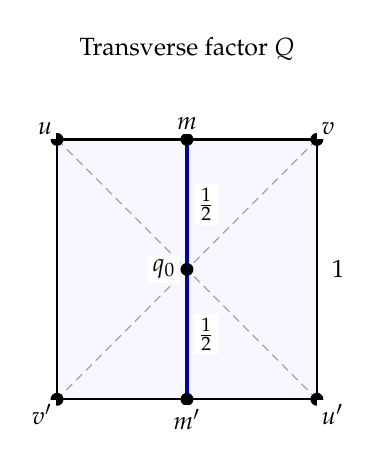
\begin{tikzpicture}[x=3.3cm,y=3.3cm,
  square vertex/.style={circle,fill=black,inner sep=1.65pt},
  square label/.style={font=\small,fill=white,inner sep=1.5pt}]
  \coordinate (u) at (-.5,.5);
  \coordinate (v) at (.5,.5);
  \coordinate (up) at (.5,-.5);
  \coordinate (vp) at (-.5,-.5);
  \coordinate (m) at (0,.5);
  \coordinate (mp) at (0,-.5);
  \coordinate (q) at (0,0);
  \fill[blue!3] (u)--(v)--(up)--(vp)--cycle;
  \draw[draw=black!40,densely dashed] (u)--(up) (v)--(vp);
  \draw[line width=.85pt] (u)--(v)--(up)--(vp)--cycle;
  \draw[draw=blue!65!black,line width=1.2pt] (m)--(mp);
  \foreach \P in {u,v,up,vp,m,mp,q}
    \node[square vertex] at (\P) {};
  \node[square label,anchor=south east] at (u) {$u$};
  \node[square label,anchor=south west] at (v) {$v$};
  \node[square label,anchor=north west] at (up) {$u'$};
  \node[square label,anchor=north east] at (vp) {$v'$};
  \node[square label,anchor=south] at (0,.52) {$m$};
  \node[square label,anchor=north] at (0,-.52) {$m'$};
  \node[square label,anchor=east] at (-.025,0) {$q_0$};
  \node[square label,anchor=west] at (.025,.25) {$\frac12$};
  \node[square label,anchor=west] at (.025,-.25) {$\frac12$};
  \node[square label,anchor=west] at (.54,0) {$1$};
  \node[font=\small] at (0,.85) {Transverse factor $Q$};
\end{tikzpicture}
\end{minipage}\hfill
\begin{minipage}[c]{.53\textwidth}
\centering
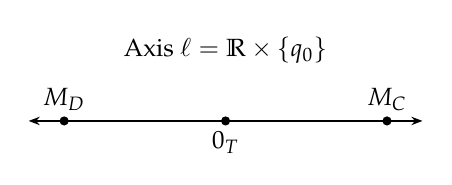
\begin{tikzpicture}[x=2.05cm,y=1cm,
  axis label/.style={font=\small,fill=white,inner sep=1.5pt}]
  \draw[{Stealth[length=4pt]}-{Stealth[length=4pt]},line width=.7pt]
    (-1.22,0)--(1.22,0);
  \foreach \x in {-1,0,1}\fill (\x,0) circle[radius=1.65pt];
  \node[axis label,anchor=south] at (-1,.07) {$M_D$};
  \node[axis label,anchor=south] at (1,.07) {$M_C$};
  \node[axis label,anchor=north] at (0,-.07) {$0_T$};
  \node[font=\small] at (0,.9) {Axis $\ell=\mathbb R\times\{q_0\}$};
\end{tikzpicture}
\par\smallskip
$P(\ell)\cong\mathbb R\times Q$\par\medskip
$M_A=2(0,m),\qquad M_B=2(0,m')$
\end{minipage}
\caption{The final contradiction takes place in the transverse factor after
splitting off the $M_C,M_D$ axis.  The cyclically ordered points $u,v,u',v'$
form a flat unit square in $Q$, with common diagonal midpoint $q_0$.
The opposite-side midpoints $m,m'$ are distance $1/2$ from $q_0$ and distance
$1$ apart.  Dilation in the original tangent cone $T$ therefore makes
$M_A=2(0,m)$ and $M_B=2(0,m')$ antipodal unit vectors.  The panels display
the two distinct factors of the parallel set.}
\label{fig:transverse-square}
\end{figure}


Finally, the full-line choices $AC,AD$ at $A$ and $BC,BD$ at $B$
give
\[
 M_A=h_{AC}\oplus h_{AD}=\delta_2(0,m),\qquad
 M_B=h_{BC}\oplus h_{BD}=\delta_2(0,m').
\]
Here $\delta_2$ is dilation in the original cone $T$; no cone
structure on $Q$ is needed.  It doubles all distances.  By
Equation~\eqref{geom:opposite-midpoints},
\[
 \norm{M_A}=\norm{M_B}=1,\qquad d_T(M_A,M_B)=2,
\]
so $\ip{M_A}{M_B}=-1$.  This contradicts
Equation~\eqref{geom:nonnegative} and proves the proposition.
\end{proof}

\section{Selection and the finite-model conclusion}\label{sec:completion}
We now assemble the arguments, keeping the order of all choices explicit.

\begin{lemma}[A deterministic diagonal sequence]\label{lem:completion-diagonal}
There is a sequence of realizations of the tables, with $n_j\to\infty$ and positive parameters $\alpha_j,\beta_j,\delta_j\to0$, such that
\begin{enumerate}[label=\textup{(\roman*)}]
\item the associated complexes $P_j$ are aspherical and have a linear letter disk-filling inequality;
\item the master match sets are nonempty and their single-field marginals tend to uniformity in total variation;
\item for every admissible pair $I,\{e\}$ and every fixed integer $t$, the common-$I$ coupling in Proposition~\ref{prop:sampling} has both of its total variation errors tending to zero along the sequence;
\item the six-letter table pair counts have uniformly vanishing relative error.
\end{enumerate}
The groups $G_j=\pi_1P_j$ are infinite.
\end{lemma}
\begin{proof}
At stage $j$, request all the admissible tests in the fixed master pattern with $1\le t\le j$. This is a finite list. Choose $\varepsilon_j>0$ small enough for Proposition~\ref{prop:sampling} for this list and for Theorem~\ref{thm:diagram}, with $\varepsilon_j<1/(400j)$, and set
\[
 \alpha_j=\delta_j=\varepsilon_j,
 \qquad \beta_j=8\varepsilon_j.
\]
These parameters satisfy $\beta_j>7\alpha_j$, and the exponent $3-\beta_j-90\delta_j$ of the master count is positive. Moreover,
\[
 j(\beta_j+90\delta_j)=98j\varepsilon_j<\frac{98}{400}<\frac12,
\]
so the explicit bound in Section~\ref{sec:sampling} preserves every overlap margin required for the finite list.

Fix these parameters. The proof of Theorem~\ref{thm:diagram} selects a finite fragment threshold, possibly depending on $j$. Its coincidence inequalities hold with probability tending to one as $n\to\infty$. For the same fixed parameters, Proposition~\ref{prop:sampling} gives the requested finite collection of sampling properties with probability tending to one. Choose $n_j>n_{j-1}$ so large that there is positive probability that all these events hold and all requested sampling errors are at most $1/j$. Select one realization in their intersection. No comparison between the fragment threshold and $n$ is needed before fixing the parameters and threshold. This proves \textup{(i)}--\textup{(iv)}.

Each $G_j$ has a quotient $C_2$ by Lemma~\ref{lem:model-presentation}. If it were finite, its universal cover would be a finite contractible CW complex, and multiplicativity of Euler characteristic would give
\[
 1=\chi(\widetilde P_j)=|G_j|\chi(P_j).
\]
Since $\chi(P_j)$ is an integer, this forces $|G_j|=1$, contrary to the quotient. Hence $G_j$ is infinite.
\end{proof}

\begin{proposition}\label{prop:completion-no-action}
For all sufficiently large $j$, the group $G_j$ in Lemma~\ref{lem:completion-diagonal} admits no geometric action on any proper complete $\CAT(0)$ space.
\end{proposition}
\begin{proof}
Suppose, more generally, that infinitely many $G_j$ admitted such actions. Restrict to that subsequence and choose one action for each of its groups. All fixed-test limits in Lemma~\ref{lem:completion-diagonal} remain valid. The action spaces, their dimensions, and their local geometries are allowed to vary.

Normalize the minimizing generator energy for each action as in Equation~\eqref{energy:normalization}. The infinitude just proved makes this energy positive. The displacement estimate and Lemma~\ref{lem:conditional-test} hold uniformly for these choices of actions. Proposition~\ref{prop:configuration} therefore supplies the limiting configuration. Proposition~\ref{prop:no-configuration} excludes it. Thus only finitely many of the selected groups can admit such actions; in particular, an instance with no action exists.
\end{proof}

\subsection{Passing to a finite simplicial model}
We record the filling transfer because the conclusion is about edge loops in a finite simplicial complex, rather than just words in a presentation.

\begin{lemma}[Finite-model filling transfer]\label{lem:completion-transfer}
Let $P$ be a finite connected CW complex with contractible universal cover. Suppose a finite presentation of $\pi_1P$ has a linear disk-filling inequality. Then $P$ has a finite connected simplicial homotopy model $K$, whose universal cover is contractible and satisfies a linear combinatorial disk-filling inequality.
\end{lemma}
\begin{proof}
A finite CW complex has a finite simplicial homotopy model of the same dimension~\cite[Theorem~2C.5]{Hatcher2002}. One construction proceeds over its finitely many cells: approximate attaching maps by simplicial maps after finite subdivisions, and use simplicial analogues of their mapping cylinders for the attachments. Let $K$ be the resulting finite simplicial model. A homotopy equivalence lifts to a homotopy equivalence of universal covers, so $\widetilde K$ is contractible.

For completeness, the linear estimate is independent of the chosen finite presentation. Choose substitutions $\phi$ from new generators to old words and $\psi$ from old generators to new words, inducing inverse group identifications. Let $L$ bound the lengths of the words $\phi(b)$, let $M$ bound the new-presentation filling areas of the finitely many substituted old relators $\psi(r)$, and let $D$ bound the filling areas of the words $b\psi(\phi(b))^{-1}$. The latter two lists consist of null words, and all three lists are finite, so these bounds exist. A new null word of length $\ell$ substitutes to an old word of length at most $L\ell$. If the old filling constant is $C_{\rm old}$, filling that word and replacing its relator cells costs at most $MC_{\rm old}L\ell$ new cells. The boundary substitutions cost at most $D\ell$ more. Thus the new filling constant is at most $MC_{\rm old}L+D$.

Apply this to the maximal-tree presentation of the finite complex $K$. Its generators correspond to the non-tree edges, and its relators to its triangular faces. A null-homotopic combinatorial edge loop in $K$ of length $\ell$ gives a null word of length at most $\ell$ in these generators after inserting paths in the fixed maximal tree. The tree has finitely many edges, so the inserted paths have uniformly bounded lengths. Fill the word linearly in the maximal-tree presentation; each relator cell is replaced by the corresponding triangular face and tree-path cancellations. The boundary collar likewise cancels the inserted tree paths with linear overhead. Thus the original loop bounds a diagram over $K$ with at most $C\ell$ triangular faces for a fixed finite $C$.

An edge loop in $\widetilde K$ projects to a null loop in $K$. Its disk diagram lifts with the chosen boundary lift, giving the required estimate in the universal cover.
\end{proof}

\begin{proof}[Proof of Theorem~\ref{thm:main}]
Choose an instance $P_j$ supplied by Proposition~\ref{prop:completion-no-action}. Its finite letter presentation has a linear disk bound by Theorem~\ref{thm:diagram}. Apply Lemma~\ref{lem:completion-transfer} to obtain $K$. Since $P_j$ has dimension two, the same-dimension construction gives a two-dimensional $K$. This proves the asserted asphericity and linear filling estimate. Its fundamental group is $G_j$, so it has the no-action property. The equivalence between a linear Dehn function and word hyperbolicity gives the final group-theoretic assertion~\cite[Exercise~III.H.2.5(5), Proposition~III.H.2.7, and Theorem~III.H.2.9]{BH1999}.

Suppose that a finite simplicial complex $L$ homotopy equivalent to $K$ admitted a compatible locally $\CAT(0)$ geodesic length metric. The metric space $L$ is compact, hence complete and locally compact. Give its universal cover the induced length metric, for which the covering map is a local isometry~\cite[Proposition~I.3.25]{BH1999}. This cover is complete: a Cauchy sequence upstairs projects to a convergent sequence downstairs; sufficiently short connecting paths force a tail into one sheet over an evenly covered neighborhood of the limit, where it converges. The Cartan--Hadamard theorem makes the cover globally $\CAT(0)$~\cite[Theorem~II.4.1(2)]{BH1999}. It is locally compact, and the length-space Hopf--Rinow theorem makes it proper~\cite[Proposition~I.3.7]{BH1999}. Its deck transformations act freely, properly and cocompactly by isometries.

The isomorphism $\pi_1L\cong\pi_1K=G_j$ therefore gives a geometric action of $G_j$ on a proper complete $\CAT(0)$ space, a contradiction. This also excludes compatible locally $\CAT(-1)$ geodesic length metrics, since a $\CAT(-1)$ space is $\CAT(0)$~\cite[Theorem~II.1.12(1)]{BH1999}.
\end{proof}

\begin{remark}
The argument makes no curvature assumption on the random complexes $P_j$. Curvature comparison is used only in a hypothetical action space, after the combinatorial filling and asphericity statements have been established. Nor is a common filling constant needed for the diagonal sequence: only the constant for the single chosen finite complex appears in Theorem~\ref{thm:main}.
\end{remark}

\bibliographystyle{plain}
\bibliography{references}
\end{document}
